\documentclass[lang=cn,10pt]{elegantbook}
\usepackage{graphicx}
\usepackage{float}
\usepackage{gensymb}
\usepackage{txfonts}
\setmainfont{TeX Gyre Termes}
\title{电磁学}



\author{ Huang}



\setcounter{tocdepth}{3}


\cover{cover.jpg}
\logo{xiao.png}
% 本文档命令
\usepackage{array}
\newcommand{\ccr}[1]{\makecell{{\color{#1}\rule{1cm}{1cm}}}}

% 修改标题页的橙色带
% \definecolor{customcolor}{RGB}{32,178,170}
% \colorlet{coverlinecolor}{customcolor}

\begin{document}
	
	\maketitle
	\frontmatter
	
	\tableofcontents
	
	\mainmatter
	\chapter{前言}
	由于时间问题,本材料无法做到面面俱到,(极化电荷、自感互感、电磁波这三个部分请配合ppt一同学习),并且有大量的习题没有敲上答案,本材料的正确使用方法是按照我在材料上写的方式学习,由于本人才疏学浅,很难保证一定不出错,如有出错请谅解。
	
	本材料的亮点之处在于目录中的重点设有超链接,点击即可学习,便于查缺补漏。此外习题训练里所选的题目均为常常会在考试中出现的题目,请务必刷完,在刷完习题的前提下,可以刷教材课后习题
	
	嗯,加油!
	\chapter{电学}
	\section{电场强度}
	\begin{introduction}
		\item 求离散电场强度
		\item 求连续电场强度(重要)
	\end{introduction}
	\subsection{求离散电场强度}
	这一部分的话,十分的简单,一般以送分题为主,主要考察库仑定律的直接应用
	\begin{theorem}[库仑定律]
		\begin{equation*}
		\overrightarrow{F_{12}}=\frac{1}{4\pi \varepsilon _0}\frac{Q_1Q_2}{{r_{12}}^2}\overrightarrow{r_{12}}\left( \varepsilon _0=8.85\times 10^{-12}C^2/\left( N\cdot m^2 \right) \right) 
		\end{equation*}
	\end{theorem}
		这一部分,会套公式就会做,没有啥要注意的,硬说的话,电场强度大小只与激发电荷有关,电偶极子这个部分,看一乐就够了
		
		\subsection{\color{red} \text{求连续电场强度}}
		
		这里所有的例题,全部要记住,做题的方法无非就是取电荷元,对其积分,简单滴很
		\begin{example}
			电荷均匀分布在一根长直细棒上,此棒电荷线密度为$\lambda$.试计算距细棒垂直距离为$a$的$P$点的场强的水平分量。已知细棒两端和$P$点连线的夹角分别为$\theta_{1}$和$\theta _{2}$
		\end{example}
		\begin{solution}
\begin{figure}[H]
	\centering
	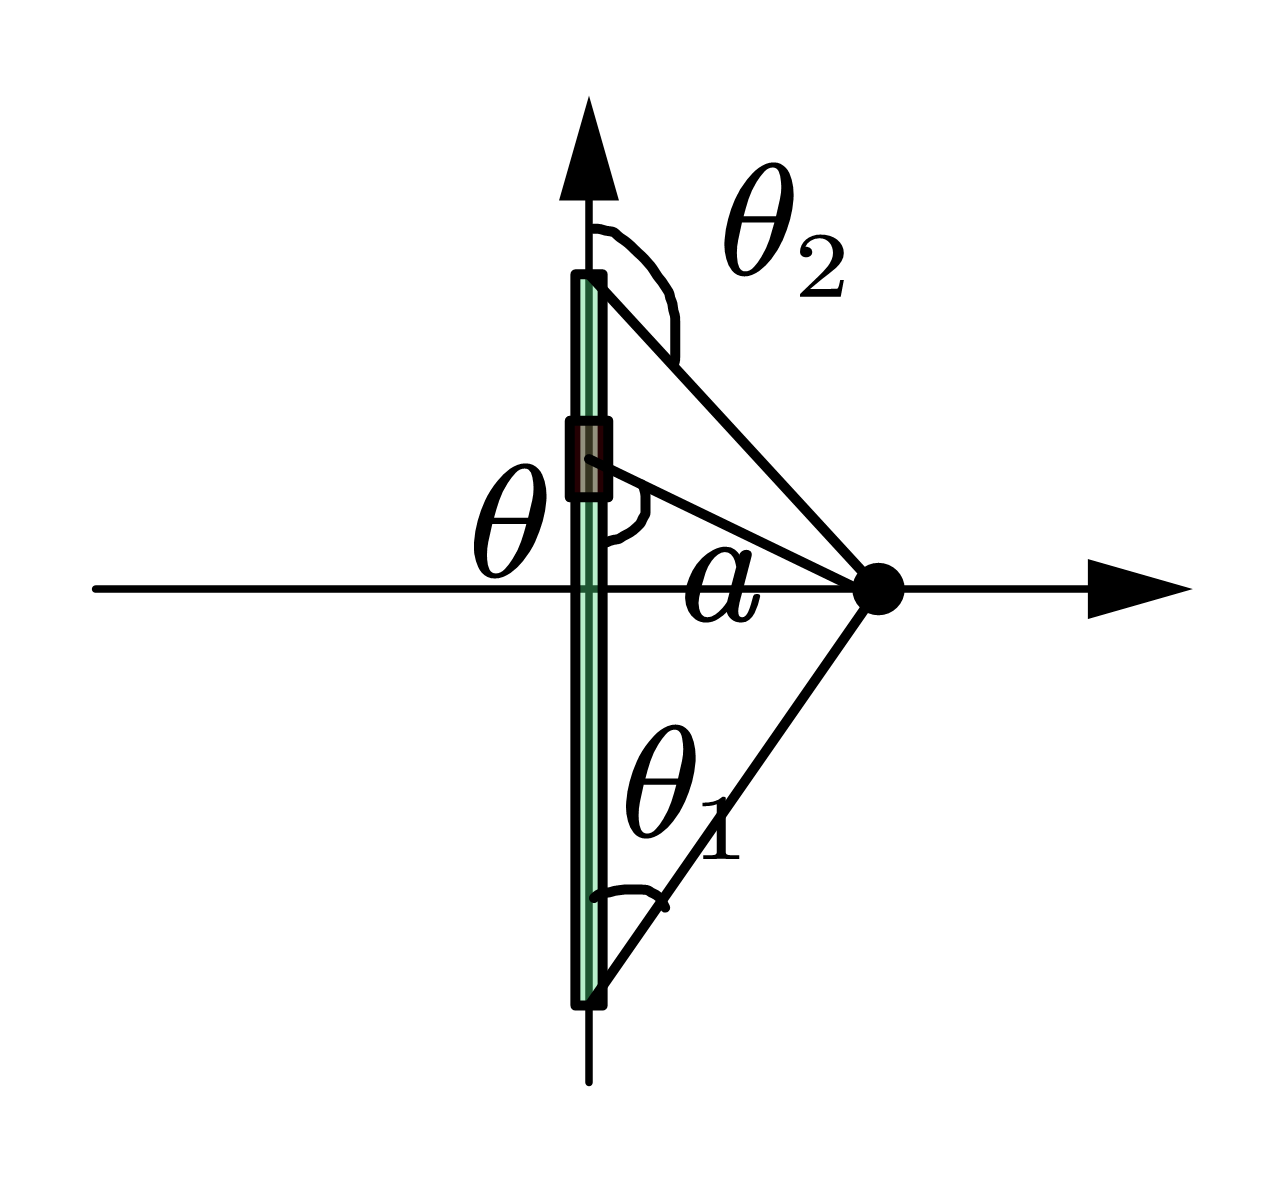
\includegraphics[width=0.3\linewidth]{image/线条}
	\caption{}
	\label{fig:}
\end{figure}
			
			如图所示,这是对线型物体的积分,我们按照套路走
			
			取电荷元$dq=\lambda dy$
			
			对单个电荷元进行分析,显然我们要对其经行电场的分解,我们有
			\begin{equation*}
				dE_x=\frac{1}{4\pi \varepsilon _0}\frac{\lambda dy}{r^2}\sin \theta 
			\end{equation*}
			
			由于$r=\frac{a}{\sin\theta},y=a\cot(\pi-\theta)=-a\cot\theta$
			
			我们有$dy=\frac{a}{\sin ^2\theta}d\theta$
			
			带入上述式子,我们可得
			\begin{equation*}
				dE_x=\frac{\lambda}{4\pi \varepsilon _0a}\sin \theta d\theta
			\end{equation*}
			
			对其积分,我们可得到一个\textbf{重要结论}
			\begin{equation*}
				E_x=\frac{\lambda}{4\pi \varepsilon _0a}\left( \cos \theta _1-\cos \theta _2 \right) 
			\end{equation*}
		\end{solution}
		\begin{note}
			当棒长为无限长的时候,我们有下述特例
			\begin{equation*}
				E_x=\frac{\lambda}{2\pi \varepsilon _0a}
			\end{equation*}
		\end{note}
		\begin{example}
			均匀带电圆环半径为$R$,带电量为$q$,求圆环轴线上一点的场强
		\end{example}
		\begin{solution}
			\begin{figure}[H]
			\centering
			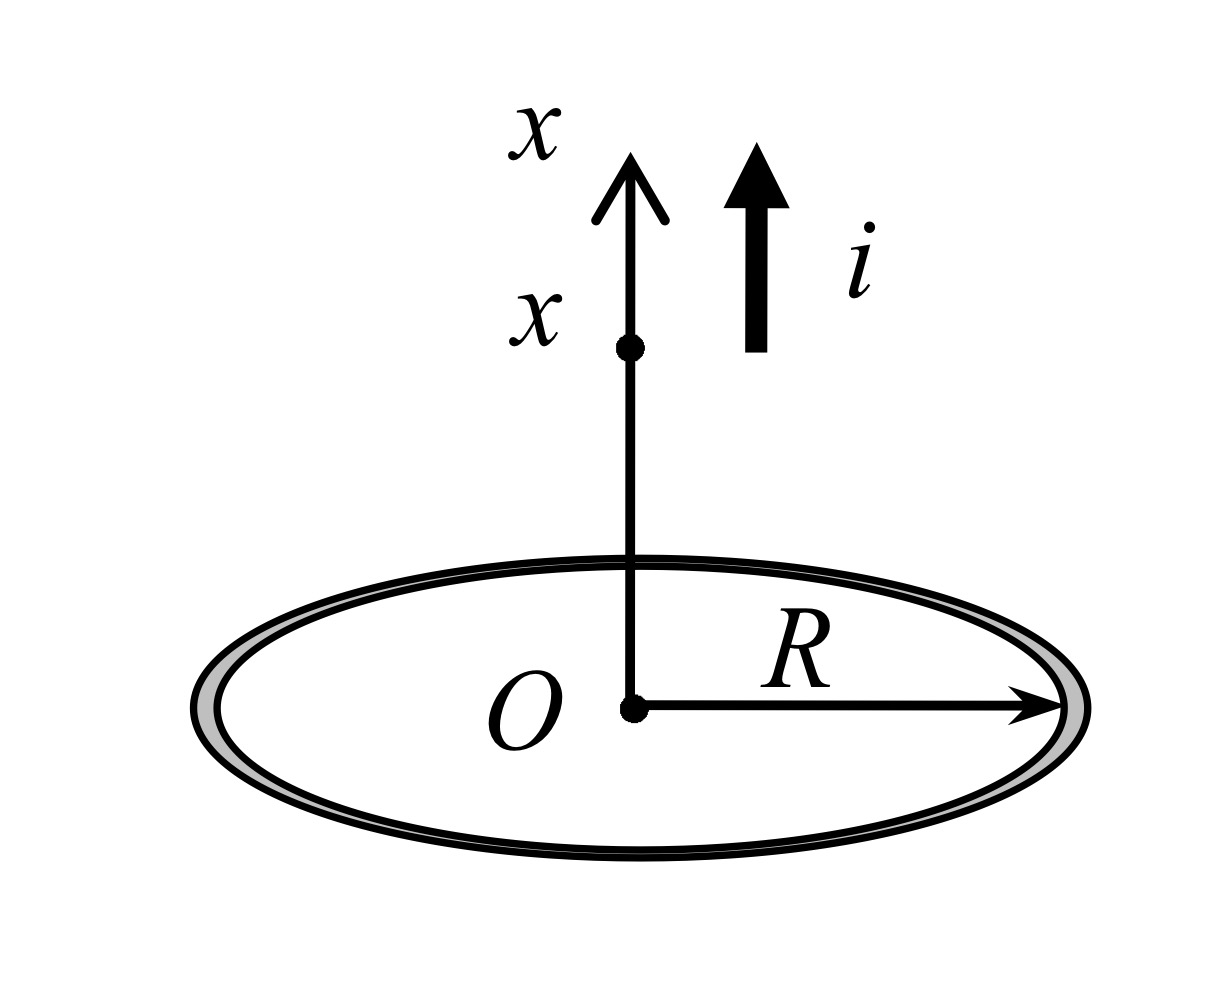
\includegraphics[width=0.3\linewidth]{image/IMG_0408(20231116-173746)}
			\caption{}
			\label{fig:img040820231116-173746}
			\end{figure}
			
			这个结论很显然,我们就不写过程了
			
			\begin{equation*}
				E=\frac{q}{4\pi \varepsilon _0}\frac{x}{\left( x^2+R^2 \right) ^{\frac{3}{2}}}
			\end{equation*}
		\end{solution}
		\begin{note}
			有个好玩的结论,在$x=\pm\frac{\sqrt{2}}{2}R$时,场强为极大值
		\end{note}
		
		有了上一题的铺垫,我们自然得出了下题的过程
		\begin{example}
			求均匀带电圆盘轴线上一点的场强,设圆盘带电量为$q$,半径为$R$
		\end{example}
		\begin{solution}
			\begin{figure}[H]
				\centering
				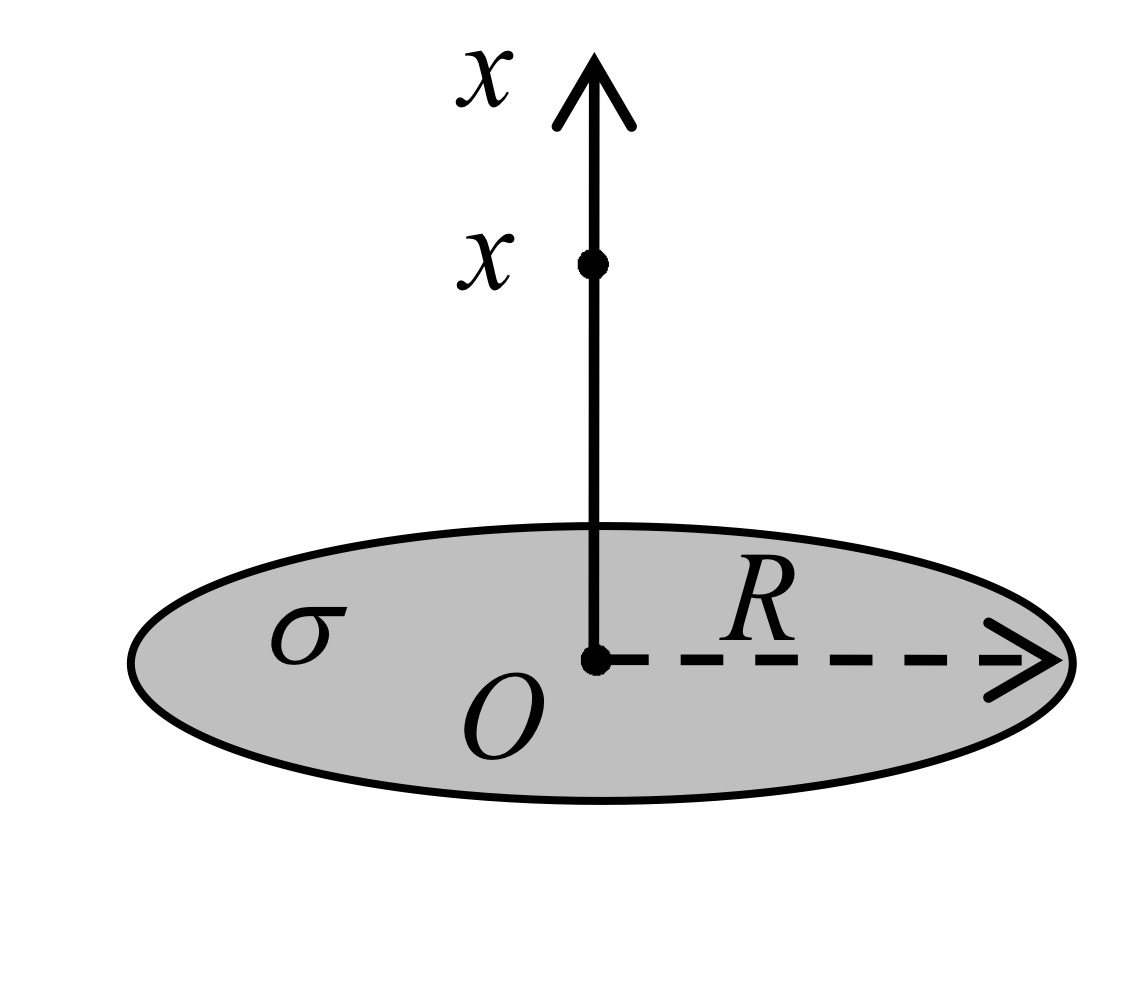
\includegraphics[width=0.3\linewidth]{image/IMG_0409(20231116-173758)}
				\caption{}
				\label{fig:img040920231116-173758}
			\end{figure}
			这个是面类型的连续体,我们采取取面电荷元的操作
			
			我们可把带电圆盘看作许多同心的圆环组成,此时我们有$dq=\sigma 2\pi r \cdot dr$
			

			此时,我们有
			\begin{equation*}
				dE=\frac{dq}{4\pi \varepsilon _0}\frac{x}{\left( x^2+R^2 \right) ^{\frac{3}{2}}}
			\end{equation*}
			
			此时积分,我们有
			\begin{equation*}
				E=\frac{\sigma}{2\varepsilon _0}\left( 1-\frac{x}{\left( x^2+R^2 \right) ^{\frac{3}{2}}} \right)
			\end{equation*}
		\end{solution}
		\begin{note}
			当圆盘无限大时,此时
			\begin{equation*}
			E=\frac{\sigma}{2\varepsilon _0}
			\end{equation*}
		\end{note}
		\section{高斯定理}
		\begin{introduction}
			\item 电场线的性质
			\item 电通量(重要)
			\item 高斯定理(重要)
			\item 环路定理(熟知)
		\end{introduction}
		\subsection{电场线的性质}
		
		\begin{note}
			1.电场线始于正电荷,终于负电荷,不会在无电荷处中断,电场线为\textbf{非闭合曲线}
			
			2.在没有电荷处同一电场,两条电场线不能相交
			
			3.电场线密处场强大,电场线疏处场强小
			
			4.沿电场线方向为电势降低的方向
		\end{note}
		\subsection{\color{red} \text{电通量}}
		\begin{definition}[电通量]
			通过任意曲面的电场线的条数称为通过这一面元的电通量
		\end{definition}
		由于通量为标量,为此我们定义一个面元矢量
		\begin{equation*}
			d\overrightarrow{S}=dS\overrightarrow{e_n}
		\end{equation*}
		
		这样我们就可以用公式来定义电通量
		\begin{equation*}
			d\varPhi =\overrightarrow{E}\cdot d\overrightarrow{S}
		\end{equation*}
		\begin{figure}[H]
		\centering
		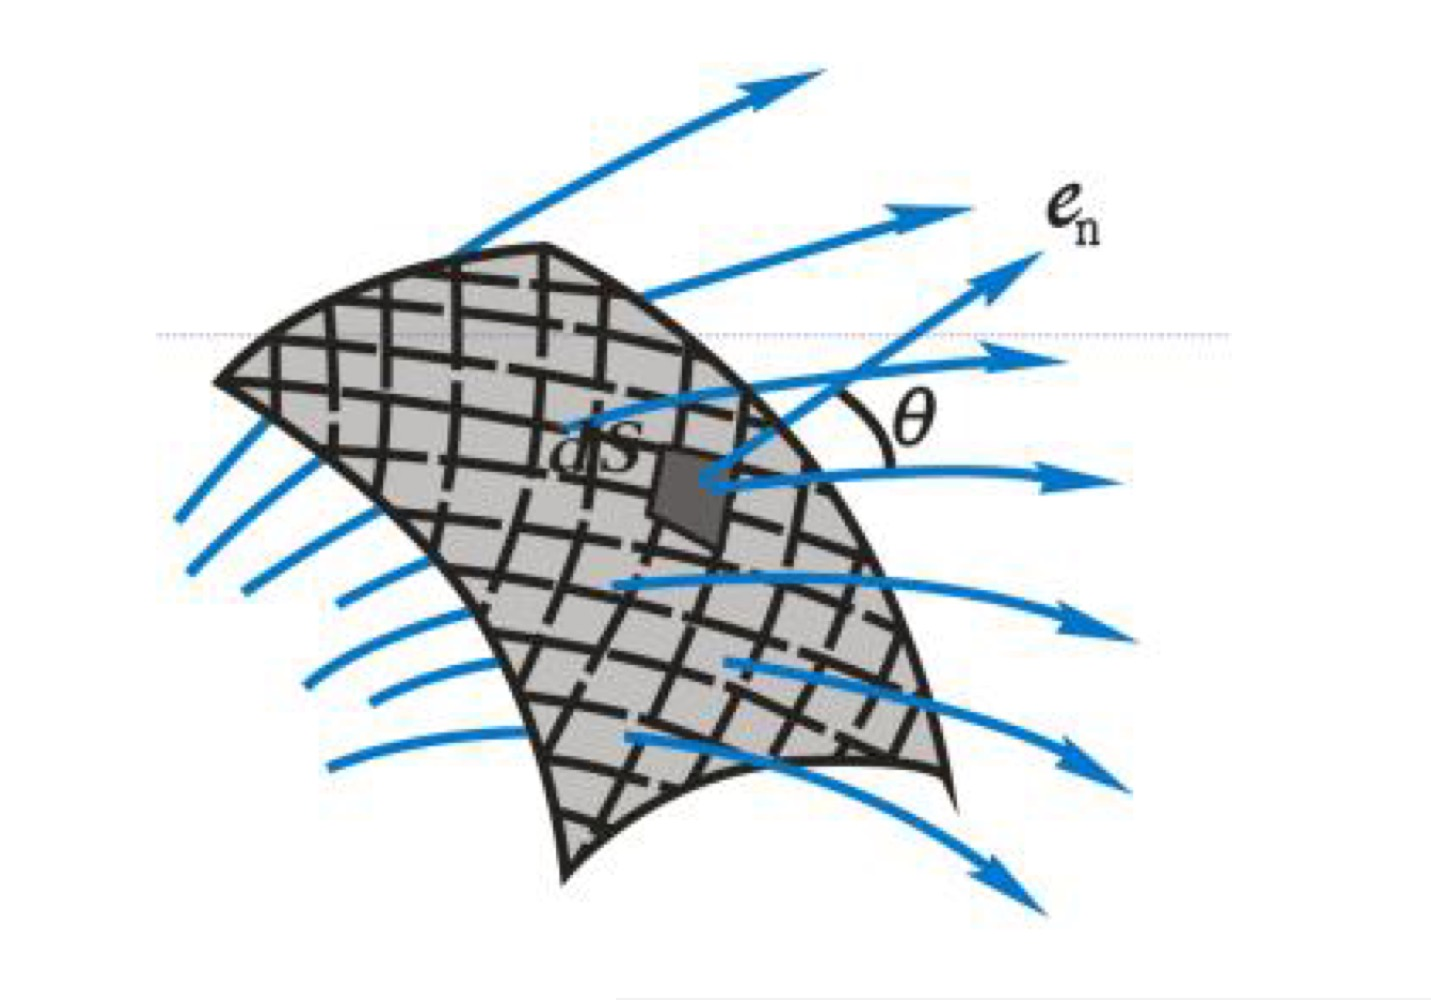
\includegraphics[width=0.3\linewidth]{image/IMG_0411(20231116-200901)}
		\caption{}
		\label{fig:img041120231116-200901}
		\end{figure}
		
		如图所示,电通量即为垂直于平面的电场线的数量,并且我们定义,\textbf{穿入闭合曲面为负通量,穿出为正通量}
		\begin{example}
			如图,在电场强度$E$的匀强电场中,有一半径为$R$的半球面,场强$E$的方向与半球面对称轴平行,穿过此半球面的电通量为
\begin{figure}[H]
	\centering
	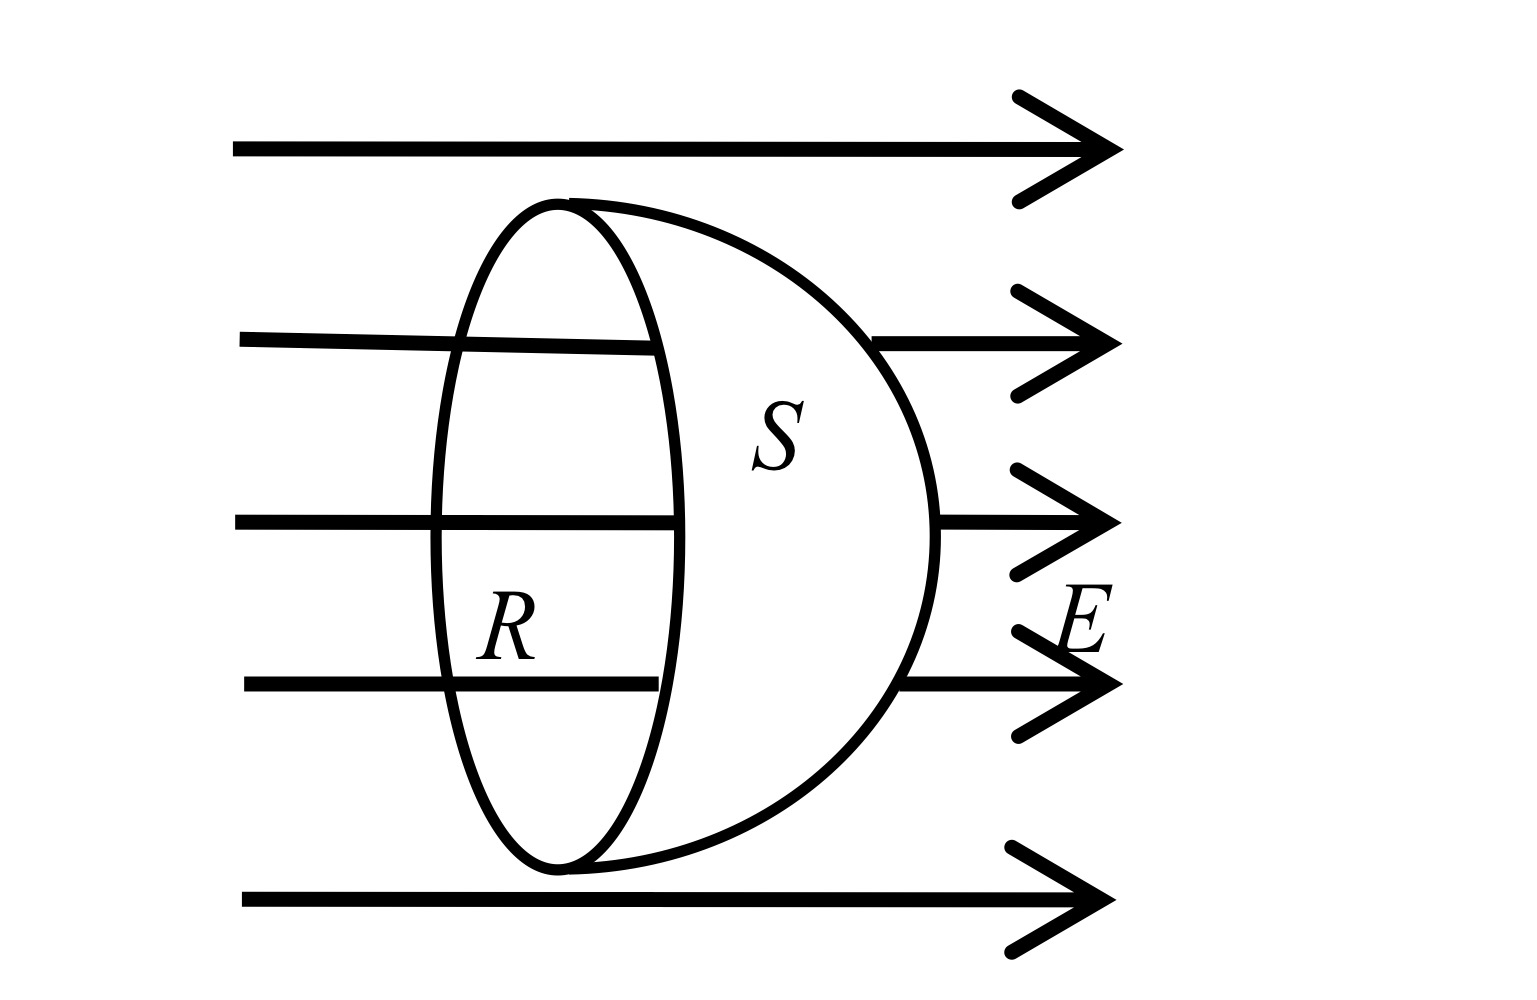
\includegraphics[width=0.18\linewidth]{image/IMG_0413(20231116-202109)}
	\caption{}
	\label{fig:img041320231116-202109}
\end{figure}
		\end{example}
		
		\begin{solution}
			电场线穿出半球面,并且半球面在垂直于电场线方向的面积为$\pi r^{2}$,于是电通量为
			\begin{equation*}
				\varPhi=E\pi r^{2}
			\end{equation*}
		\end{solution}
		\begin{example}
			有一半径为$R$的半球面如图所示,通过半球面的电通量为
\begin{figure}[H]
	\centering
	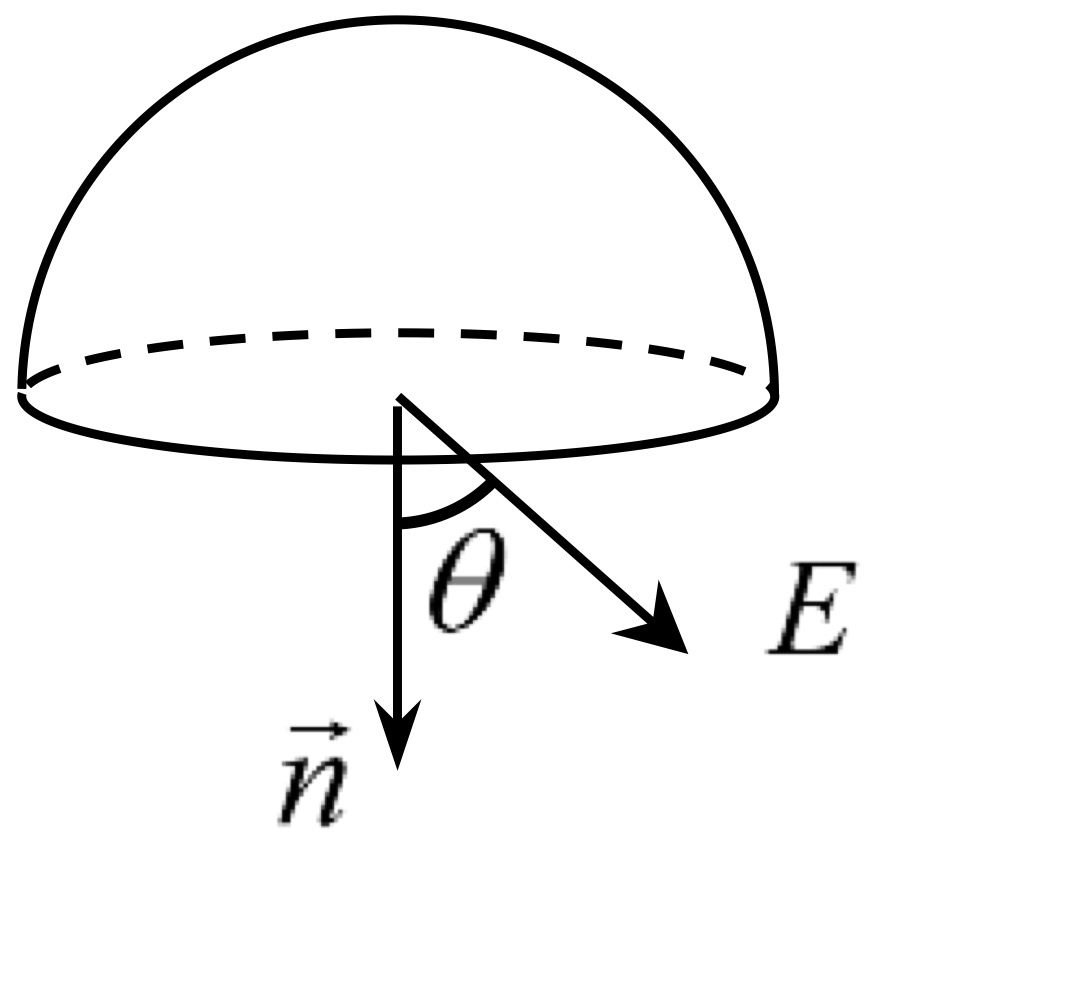
\includegraphics[width=0.18\linewidth]{image/IMG_0414(20231116-202133)}
	\caption{}
	\label{fig:img041420231116-202133}
\end{figure}
		\end{example}
		\begin{solution}
			电场线穿入半球面,实际有用的电场线为在法线上的投影,并且半球面在垂直于法线方向的面积为$\pi r^{2}$,于是电通量为
			\begin{equation*}
				\varPhi=-E\pi r^{2}
				\cos\theta
			\end{equation*}
		\end{solution}
		\subsection{\color{red} \text{高斯定理}}
		\begin{theorem}[高斯定理]
			静电场中穿过任一曲面的电通量等于闭合曲面内电荷的代数和除以真空的介电常数$\varepsilon_{0}$,
			
			用公式表示就是
			\begin{equation*}
				\oiint{\overrightarrow{E}\cdot d\overrightarrow{S}}=\frac{\sum_V{q_i}}{\varepsilon _0}=\frac{\oiiint\limits_V{\rho _edV}}{\varepsilon _0}
			\end{equation*}
			$V$是闭面$S$所包围的空间
		\end{theorem}
		\begin{note}
			此时我们如果用高斯公式
			\begin{equation*}
				\oiint{\overrightarrow{E}\cdot d\overrightarrow{S}}=\oiiint\limits_V{\nabla \cdot \overrightarrow{E}dV}
			\end{equation*}
			
			可得到
			\begin{equation*}
				\nabla \cdot \overrightarrow{E}=\frac{\rho _e}{\varepsilon _0}
			\end{equation*}
			表明$E$的散度不为0,即静电场是有源场
		\end{note}
		\begin{remark}
			若高斯面上的场强处处为零,则高斯面内无净电荷
		\end{remark}
		\begin{remark}
			电通量与高斯面内电荷有关,与电荷的位置以及高斯面外电荷无关
		\end{remark}
		\begin{remark}
			高斯面上的场强,受面内和面外电荷的共同影响
		\end{remark}
		
		下面的例题中的结论,请\textbf{务必记住},记不住的话,\textbf{最少要会推}
		\begin{example}
			半径$R$、带电量为$q$的均匀带电球体,计算球体内外的电场强度
		\end{example}
		\begin{solution}
			\begin{equation*}
				\ointctrclockwise{\overrightarrow{E}\cdot d\overrightarrow{S}}=\frac{\sum_V{q_i}}{\varepsilon _0}
			\end{equation*}
			
			解得
			\begin{equation*}
				\overrightarrow{E}=\frac{\sum_V{q_i}}{4\pi \varepsilon _0r^2}
			\end{equation*}
			
			又因为体密度为
			\begin{equation*}
				\rho =\frac{q}{V}=\frac{q}{\frac{4}{3}\pi R^3}=\frac{3q}{4\pi R^3}
			\end{equation*}
			
			$r<R$时,$\sum_V{q_i}=\rho V_{r}=\frac{3q}{4\pi R^3}\frac{4}{3}\pi r^3=\frac{qr^{3}}{R^{3}}$
			
			解得
			\begin{equation*}
				E=\frac{qr}{4\pi\varepsilon_{0}R^{3}}
			\end{equation*}
			
			$r>R$时,$\sum_V{q_i}=q$
			\begin{equation*}
				E=\frac{q}{4\pi\varepsilon_{0}r^{2}}
			\end{equation*}
		\end{solution}
		
		\begin{example}
			求半径为$R$,线密度为$\lambda$的无限长均匀圆柱面电荷的电场分布
		\end{example}
		\begin{solution}
			\begin{equation*}
				\ointctrclockwise{\overrightarrow{E}\cdot d\overrightarrow{S}}=\frac{\sum_V{q_i}}{\varepsilon _0}
			\end{equation*}
			
			$r<R$时,$\sum_V{q_i}=\frac{\lambda h}{\pi R^{2}h}\cdot \pi r^{2}h=\frac{r^{2}}{R^{2}}\lambda h$
			
			解得
			\begin{equation*}
				E=\frac{\lambda r}{2\pi \varepsilon_{0}R^{2}}
			\end{equation*}
			
			$r>R$时,$\sum_V{q_i}=\lambda h$
			
			解得
			\begin{equation*}
				E=\frac{\lambda}{2\pi \varepsilon_{0} r}
			\end{equation*}
		\end{solution}
		\begin{example}
			求半径为$R$,面密度为$\lambda$的均匀圆柱面电荷的电场分布
		\end{example}
		\begin{solution}		
			\begin{equation*}
				\ointctrclockwise{\overrightarrow{E}\cdot d\overrightarrow{S}}=\frac{\sum_V{q_i}}{\varepsilon _0}
			\end{equation*}
			
			$r<R$时,$\sum_V{q_i}=0,E=0$
			
			$r>R$时,$\sum_V{q_i}=
			\sigma 2\pi Rh$
			
			解得
			\begin{equation*}
				E=\frac{\sigma R}{\varepsilon_{0}r}
			\end{equation*}
		\end{solution}
		\subsection{环路定理(会用就行)}
		\begin{theorem}[环路定理]
			在静电场中,场强沿任意闭合路径的线积分等于0
			
			用公式表达就是
			\begin{equation*}
				\ointclockwise{\overrightarrow{E}\cdot d\overrightarrow{l}}=0
			\end{equation*}
		\end{theorem}
		\begin{note}
			若采用斯托克斯定理
			\begin{equation*}
				\ointclockwise{\overrightarrow{E}\cdot d\overrightarrow{l}}=\oiint{\left( \nabla \times \overrightarrow{E} \right)}\cdot d\overrightarrow{S}=0
			\end{equation*}
			可得
			\begin{equation*}
				\nabla \times \overrightarrow{E}=0
			\end{equation*}
			表明静电场的旋度为0,即说明静电场不闭合
		\end{note}
		\section{电势、电势能}
		\begin{introduction}
			\item 电势能(重要)
			\item 电势(重要)
			\item 电势和电场关系(熟知)
		\end{introduction}
		\subsection{\color{red} \text{电势能}}
		\begin{definition}[电势能]
			电荷在某点的电势能等于将此电荷沿任意路径移到电势能零点的过程电场力所做的功
		\end{definition}
		\begin{note}
			电势能是个相对的量,必须要选择一个零势能点作为参考
		\end{note}
	
		\subsection{\color{red} \text{电势}}
		\begin{definition}[电势]
			把单位正电荷从场点$a$经过任意路径移到零电势参考点时电场力所做的功。也等于单位正电荷在$a$点所具有的电势能。
			
			用公式表示就是
			\begin{equation*}
				U_a=\int\limits_a^{\text{零点}}{\overrightarrow{E}\cdot \overrightarrow{dl}}
			\end{equation*}
		\end{definition}
		\begin{remark}
			电势是标量,有大小正负,无方向
		\end{remark}
		\begin{remark}
			零势能点可以任意选取,不同的势能点对应的电势不同
		\end{remark}
		\subsubsection{求离散型电势}
		
		这个部分我们只需要知道一个公式
		\begin{equation*}
			U=\frac{q}{4\pi\varepsilon_{0}r}
		\end{equation*}
		剩下的硬套就行了
			\begin{example}
			如图所示,在$A$、$B$两点有电量分别为$+q,-q$的点电荷,$A$、$B$间的距离为$2R$,现在将另一正试验点电荷$q_{0}$从$O$点经半圆弧移动到$C$点,电场力所做的功为?
			\begin{figure}[H]
				\centering
				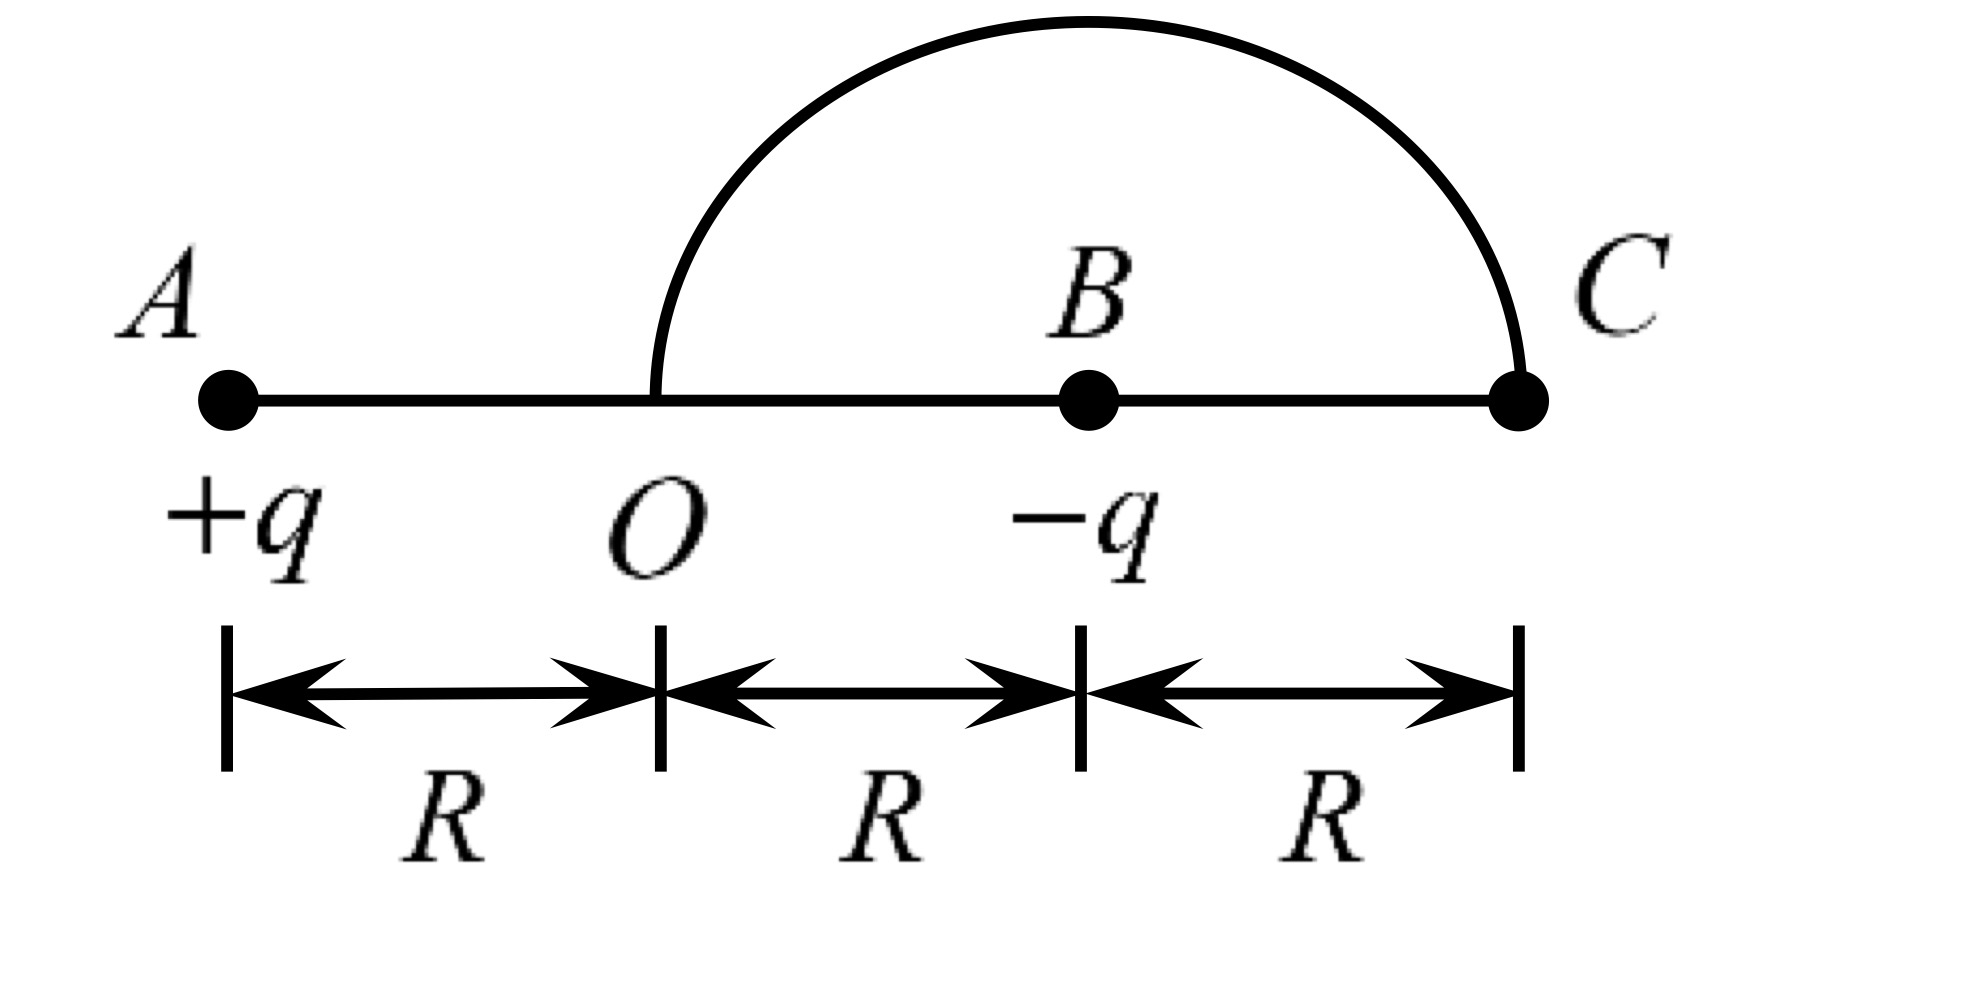
\includegraphics[width=0.18\linewidth]{image/IMG_0415(20231116-231400)}
				\caption{}
				\label{fig:img041520231116-231400}
			\end{figure}
		\end{example}
		\begin{solution}
			
			$O$点电势$U_{O}=\frac{q}{4\pi\varepsilon_{0}R}+\frac{-q}{4\pi\varepsilon_{0}R}$=0
			
			$C$点电势$U_{O}=\frac{q}{4\pi\varepsilon_{0}3R}+\frac{-q}{4\pi\varepsilon_{0}R}$=$\frac{-q}{6\pi\varepsilon_{0}R}$
			
			电场力做功$q_{0}U_{OC}=\frac{q_{0}q}{6\pi\varepsilon_{0}R}$
		\end{solution}
		\subsubsection{求连续型电势}
		这个部分我们只需要知道一个公式,取电荷元
		\begin{equation*}
			dU=\frac{dq}{4\pi\varepsilon_{0}r}
		\end{equation*}
		
		然后对其积分即可
		\begin{example}
			一均匀带点半圆环,半径为$R$,带电量为$+Q$,求环心处的电势
\begin{figure}[H]
	\centering
	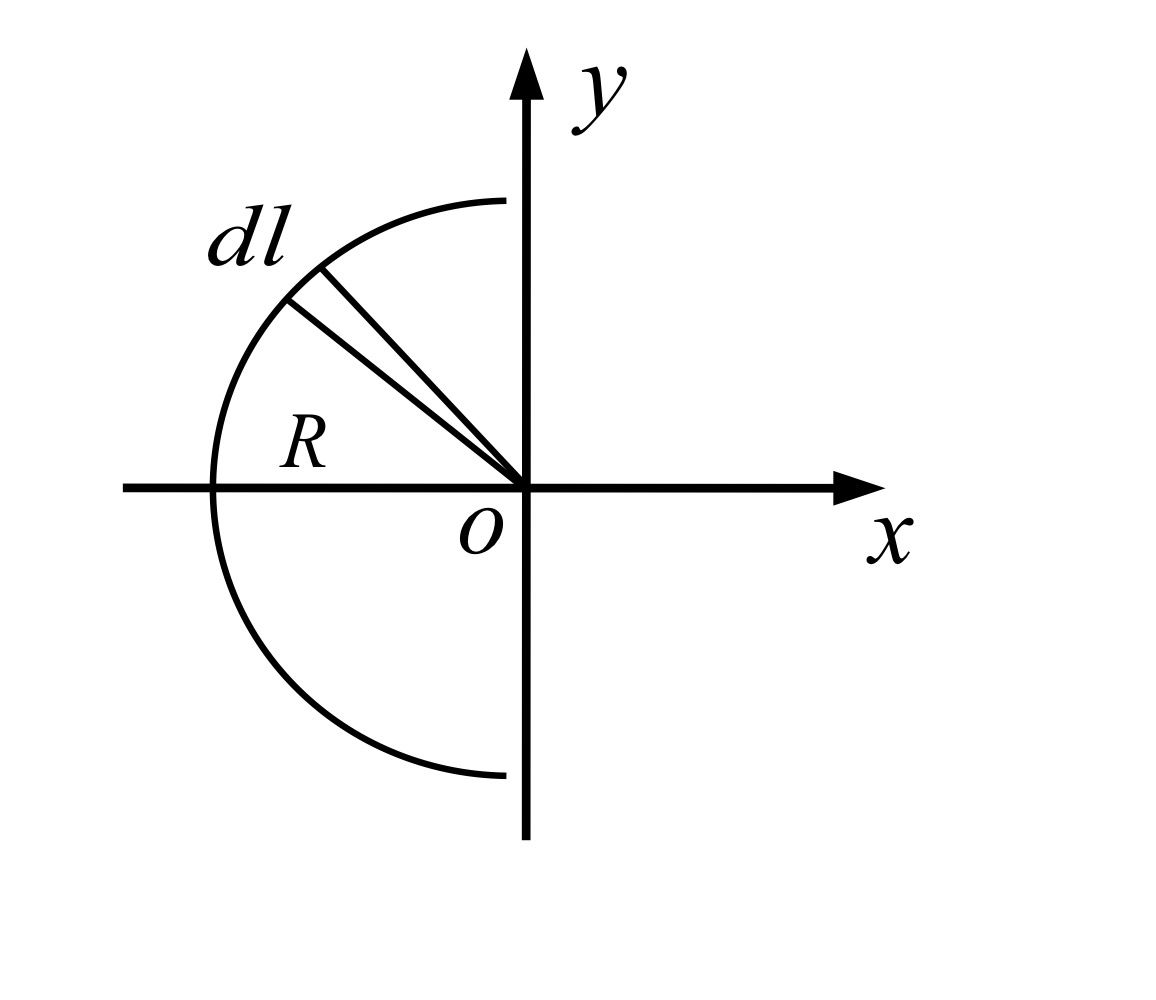
\includegraphics[width=0.18\linewidth]{image/IMG_0416(20231117-173212)}
	\caption{}
	\label{fig:img041620231117-173212}
\end{figure}
		\end{example}
		\begin{solution}
			这是对线的积分,我们要取电荷线密度
			
			显然电荷线密度$\lambda=\frac{Q}{\pi R},dq=\lambda dl$
			
			于是
			\begin{equation*}
				dU=\frac{dq}{4\pi\varepsilon_{0}r}=\frac{\lambda dl}{4\pi\varepsilon_{0}r}=\frac{Q}{\pi R}\frac{ dl}{4\pi\varepsilon_{0}r}
			\end{equation*}
		
			对电荷元积分可得
			\begin{equation*}
				U=\int\limits_0^{\pi r}{\frac{Q}{\pi R}\frac{dl}{4\pi \varepsilon _0r}}=\frac{Q}{4\pi \varepsilon _0R}
			\end{equation*}
		\end{solution}
		\begin{example}
			一绝缘细棒弯成半径为$R$的四分之一圆形环,使之均匀带正电,电荷线密度为$+\lambda$,设无穷远处为零电势点,则在四分之一圆环圆心$O$处的电势为
		\end{example}
		\begin{solution}
			同上,我们可解的$U=\frac{\lambda}{8\varepsilon_{0}}$
		\end{solution}
		\begin{note}
			若圆环、半圆环、或者部分圆环,只需要求出总电量$Q$然后直接带入电势公式即可求出在圆心的电势
		\end{note}
		\subsubsection{已知场强求对应电势}
		这里我们就需要用到定义
		\begin{equation*}
			U_a=\int\limits_a^{\text{零点}}{\overrightarrow{E}\cdot \overrightarrow{dl}}
		\end{equation*}
		直接计算即可,下面这道例题十分经典,结论\textbf{可以记住}
		\begin{example}
			求电荷量为$q$的均匀带电球壳内外电势分布
		\end{example}
		\begin{solution}
			由高斯定理可求得
			
			$r<R,E=0$
			
			$r>R,E=\frac{q}{4\pi \varepsilon_{0}r^{2}}$
			
			$r<R$时
			\begin{equation*}
				U=\int\limits_r^R{0dr}+\int\limits_R^{\infty}{\frac{q}{4\pi \varepsilon _0r^2}dr}=\frac{q}{4\pi \varepsilon _0R}
			\end{equation*}
			
			$r>R$时
			\begin{equation*}
				U=\int\limits_r^{\infty}{\frac{q}{4\pi \varepsilon _0r^2}dr}=\frac{q}{4\pi \varepsilon _0r}
			\end{equation*}
		\end{solution}
		\subsection{电势和电场关系}
		这里的关系,用公式来表示即为
		\begin{equation*}
			\overrightarrow{E}=-\left( \frac{\partial U}{\partial x},\frac{\partial U}{\partial y},\frac{\partial U}{\partial z} \right)
		\end{equation*}
		\begin{remark}
			电场线密的地方电场强度越大
		\end{remark}
		\begin{remark}
			电势沿电场线方向减小
		\end{remark}
		\begin{remark}
			某点电势随电势零点不同而不同
		\end{remark}
		\begin{remark}
			描述静电场性质的两个基本物理量为电场强度和电势
		\end{remark}
		\section{导体}
		\begin{introduction}
			\item 静电平衡(重要)
			\item 导体的场强和电势(重要)
		\end{introduction}
		\subsection{\color{red} \text{静电平衡}}
		\begin{definition}[静电平衡]
			在电场中,导体的内部和表面都没有电荷定向移动的状态
		\end{definition}
		\begin{note}
			静电平衡条件:
			
			1.导体内部场强处处为0
			
			2.与导体表面紧邻的外表面处场强与导体表面正交
		\end{note}
		\begin{remark}
			静电平衡的导体是等势体,表面是等势面,但场强并非处处相等
		\end{remark}
		\begin{remark}
			导体表面电场强度为$E=\frac{\sigma}{\varepsilon_{0}}$
		\end{remark}
		\begin{remark}
			导体表面曲率越大(越尖锐),电荷密度越大
		\end{remark}
		\begin{remark}
			静电平衡的导体,电荷分布在表面
		\end{remark}
		下面这一题,将静电感应和静电平衡的考点全搞出来了
		\begin{example}
			半径为$R$的金属球与地相连接,在与球心相距$d=2R$处有一点电荷$q>0$,问球上的感应电荷$q'$=?
		\end{example}
		\begin{solution}
			由静电平衡导体是个等势体,球上电势处处为0
			
			对球心,有
			\begin{equation*}
				\frac{q'}{4\pi \varepsilon _0R}+\frac{q}{8\pi \varepsilon _0R}=0
			\end{equation*}
			
			解得
			\begin{equation*}
				q'=-\frac{q}{2}
			\end{equation*}
		\end{solution}
		\subsection{\color{red} \text{导体的场强和电势}}
		\begin{example}
			在点电量为$q$、半径为$R_{1}$的金属球壳外同心放置一个内外半径为$R_{2},R_{3}$的金属球壳。
			
			1、求外球壳上电荷及电势分布
			
			2、把外球接地后再绝缘,求外球上的电荷分布及球壳内外的电势分布
			
			3、再把内球接地,求内球上的电荷分布及球壳的电势
			
			\begin{figure}[H]
				\centering
				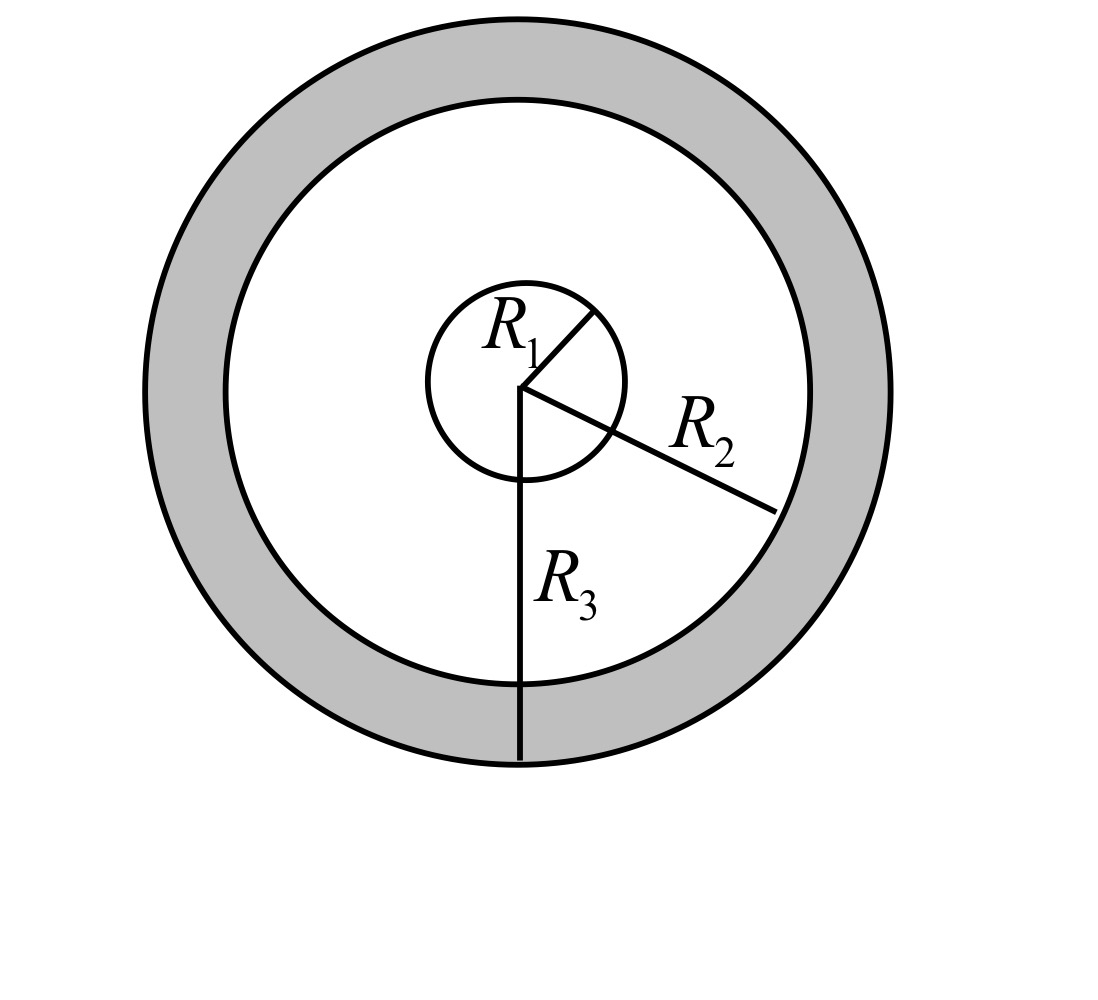
\includegraphics[width=0.2\linewidth]{image/IMG_0417(20231117-191724)}
				\caption{}
				\label{fig:img041720231117-191724}
			\end{figure}
		\end{example}
		\begin{solution}
			1. 由静电平衡,内表面电荷$q_{2}=-q$,$q_{3}=q$
			
			$r<R_{1}$时,
			\begin{equation*}
				U_1=\frac{q}{4\pi \varepsilon _0R_1}+\frac{-q}{4\pi \varepsilon _0R_2}+\frac{q}{4\pi \varepsilon _0R_3}
			\end{equation*}
			
			$R_{1}<r<R_{2}$时
			\begin{equation*}
				U_2=\frac{q}{4\pi \varepsilon _0r}+\frac{-q}{4\pi \varepsilon _0R_2}+\frac{q}{4\pi \varepsilon _0R_3}
			\end{equation*}
			
			$R_{2}<r<R_{3}$时
			\begin{equation*}
				U_3=\frac{q}{4\pi \varepsilon _0r}+\frac{-q}{4\pi \varepsilon _0r}+\frac{q}{4\pi \varepsilon _0R_3}=\frac{q}{4\pi \varepsilon _0R_3}
			\end{equation*}
			
			$	r>R_{3}$
			\begin{equation*}
				U_4=\frac{q}{4\pi \varepsilon_0 r}
			\end{equation*}
			
			2.接地会导致接地的那一部分为电势为0,注意,不是电荷为0,在外球接地后,会导致外球电势为0,使得其激发电荷全部转移到大地,此时$q_{3}=0$
			
			$r<R_{1}$时,
			\begin{equation*}
				U_1=\frac{q}{4\pi \varepsilon _0R_1}+\frac{-q}{4\pi \varepsilon _0R_2}
			\end{equation*}
			
			$R_{1}<r<R_{2}$时
			\begin{equation*}
				U_2=\frac{q}{4\pi \varepsilon _0r}+\frac{-q}{4\pi \varepsilon _0R_2}
			\end{equation*}
			
			$R_{2}<r<R_{3}$时
			\begin{equation*}
				U_3=\frac{q}{4\pi \varepsilon _0r}+\frac{-q}{4\pi \varepsilon_0 r}=0
			\end{equation*}
			
			$	r>R_{3}$
			\begin{equation*}
				U_4=0
			\end{equation*}
			
			3. 当把内球接地时,接地的那一处电势为0,但不一定全部电荷移动到大地,但还是遵守电荷守恒
			
			即
			\begin{equation*}
				q'_{2}+q'_{3}=-q,q'_{2}=-q'_{1}
			\end{equation*}
			
			接地的那一处电势为0,列电势方程,即可解得
			\begin{equation*}
				q'_{3}=\frac{\left( R_2R_3-R_1R_3 \right) q}{R_1R_3-R_2R_3-R_1R_2}
			\end{equation*}
			
			带入解得
			\begin{equation*}
				U_3=\frac{1}{4\pi \varepsilon _0R_3}\frac{\left( R_2R_3-R_1R_3 \right) q}{R_1R_3-R_2R_3-R_1R_2}
			\end{equation*}
		\end{solution}
		\section{电介质}
		\begin{introduction}
			\item 电介质的极化(了解)
			\item 极化强度矢量(了解)
			\item 介质中的高斯定理(重要)
		\end{introduction}
		\subsection{电介质的极化}
		字太多了,看ppt去
		\subsection{极化强度矢量}
		这一部分自己看ppt,太鸡肋了,结论记一下就行了		
		\subsection{\color{red}\text{介质中的高斯定理}}       
		\begin{theorem}[介质中的高斯定理]
			通过任意曲面的电位移通量等于该曲面内所包围的自由电荷的代数和
			
			用公式表示即为
			\begin{equation*}
				\oiint_S{\overrightarrow{D}\cdot d\overrightarrow{S}}=\sum_S{q_i},\text{其中}\overrightarrow{D}=\varepsilon _0\varepsilon _r\overrightarrow{E}
			\end{equation*}
		\end{theorem}              这个做题的方法和在真空中的高斯定理一模一样,都得想办法构造出一个高斯面,算通量,单独考没什么特别出彩的考点,但其一旦和后面的电容器和电场能量结合起来,那就十分的辉煌,这个我们放在习题训练里
		
		\begin{example}
			在半径为$R_{1}$的金属球之外包有一层外半径为$R_{2}$的均匀电介质球壳,介质的相对介电常数为$\varepsilon_{r}$,金属球带电$Q$,试求
			
			1.电介质内外的场强
			
\begin{figure}[H]
	\centering
	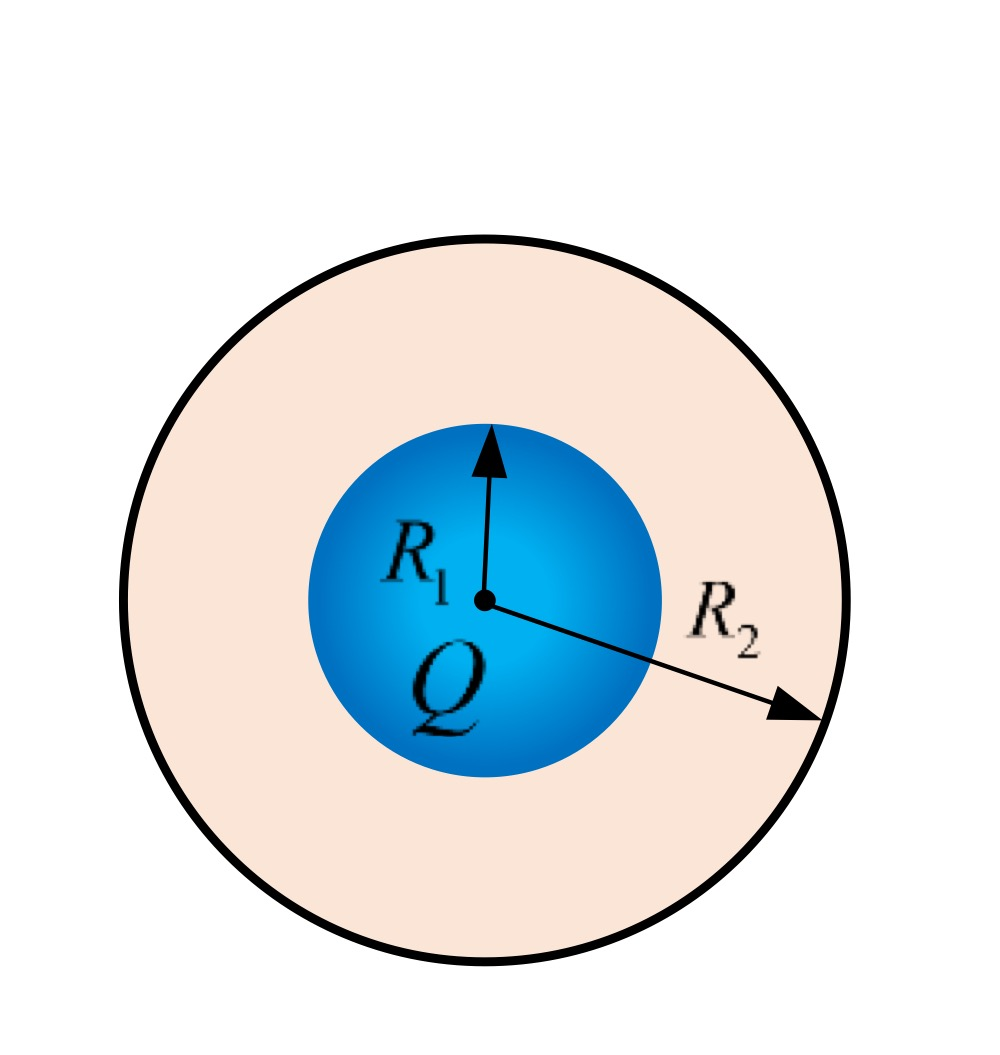
\includegraphics[width=0.18\linewidth]{image/IMG_0418(20231118-125659)}
	\caption{}
	\label{fig:img041820231118-125659}
\end{figure}
		\end{example}
		 \begin{solution}
		 	
		 	(1)
		 	\begin{equation*}
		 		\oiint_S{\overrightarrow{D}\cdot d\overrightarrow{S}}=\sum_S{q_i}
		 	\end{equation*}
		 	解得
		 	
		 	\begin{equation*}
		 		\overrightarrow{E}=\frac{\overrightarrow{D}}{\varepsilon _0\varepsilon _r}=\frac{\sum{q}}{4\pi r^2\varepsilon _0\varepsilon _r}
		 	\end{equation*}
		 	
		 	$r<R_{1},\sum{q}=0,\varepsilon_{r}=\varepsilon_{r},E=0$
		 	
		 	$R_{1}<r<R_{2},\sum{q}=Q,\varepsilon_{r}=\varepsilon_{r},E=\frac{Q}{4\pi r^2\varepsilon _0\varepsilon _r}$
		 	
		 	$r>R_{2},\sum{q}=Q,\varepsilon_{r}=1,E=\frac{Q}{4\pi r^2\varepsilon _0}$
		 	
		 	
		 \end{solution}    
		\section{电容}
		\begin{introduction}
			\item 电容器(重要)
			\item 常见电容器的电容
			\item 电容的计算方法(重要)
		\end{introduction}
		\subsection{\color{red}\text{电容器}}
		\begin{definition}[电容]
			反映孤立导体储存电荷能力大小的物理量
			
			用公式表示就是
			\begin{equation*}
				C=\frac{Q}{U}
			\end{equation*}
		\end{definition}
		\begin{remark}
			常用换算$1\mu F=10^{-6}F,1pF=10^{-12}F$
		\end{remark}
		\begin{remark}
		极板间相互作用力$F=\frac{1}{2}EQ$
		\end{remark}
		
		\subsection{常见电容器的电容}
		\begin{tabular}{|c|c|c|c|c|c|}
			\hline
		常见电容器	& 平行板电容器 & 圆柱形电容器 &球形电容器  \\
			\hline
		真空中	&$C=\frac{\varepsilon _0S}{d}$  & $C=\frac{2\pi \varepsilon _0l}{\ln \frac{R_B}{R_A}}$ &$C=4\pi \varepsilon _0\frac{R_AR_B}{R_B-R_A}$    \\
			\hline
		含介质$\varepsilon_{r}$	&$C=\frac{\varepsilon _0\varepsilon_{r} S}{d}$  & $C=\frac{2\pi \varepsilon _0\varepsilon _{r}l}{\ln \frac{R_B}{R_A}}$ &$C=4\pi \varepsilon _0\varepsilon_{r}\frac{R_AR_B}{R_B-R_A}$    \\
			\hline
		\end{tabular}
		\subsection{\color{red}\text{电容的计算方法}}	
		\begin{note}
			1.设电量
			
			2.求场强
			
			3.算电势差
			
			4.套定义
		\end{note}	
		\begin{example}
			求面积为$S$,两极板间距离为$d$的平行板电容器的电容
			
\begin{figure}[H]
	\centering
	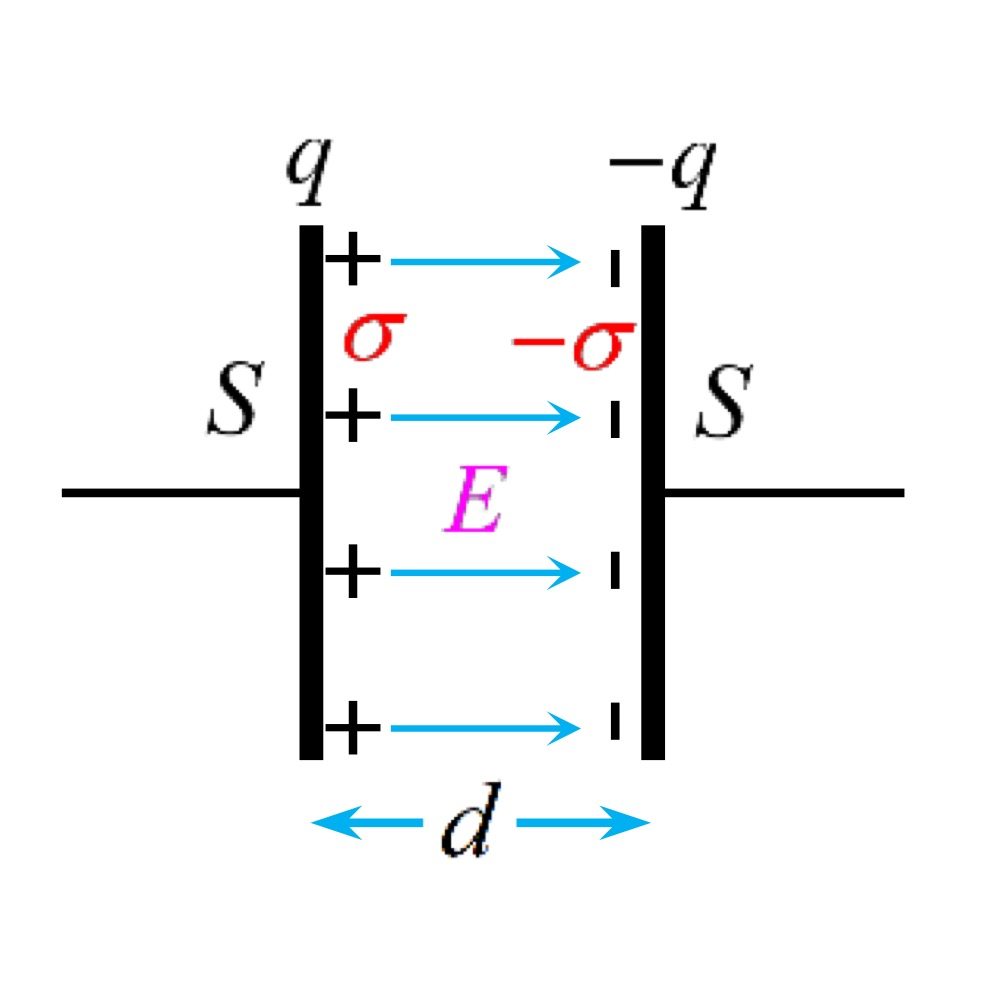
\includegraphics[width=0.18\linewidth]{image/IMG_0420(20231118-140226)}
	\caption{}
	\label{fig:img042020231118-140226}
\end{figure}
		\end{example}
		\begin{solution}
			
			1.设电量:设左右两版电量为$+q,-q$
			
			2.求场强:$E=\frac{\sigma}{\varepsilon_{0}}=\frac{q}{S\varepsilon_{0}}$
			
			3.算电势差:$U_{ab}=Ed=\frac{qd}{S\varepsilon_{0}}$
			
			4.套定义:$C=\frac{q}{U}=\frac{\varepsilon_{0}S}{d}$
		\end{solution}
		\begin{example}
			求内半径为$R_{A}$,外半径为$R_{B}$的球形电容器的电容
\begin{figure}[H]
	\centering
	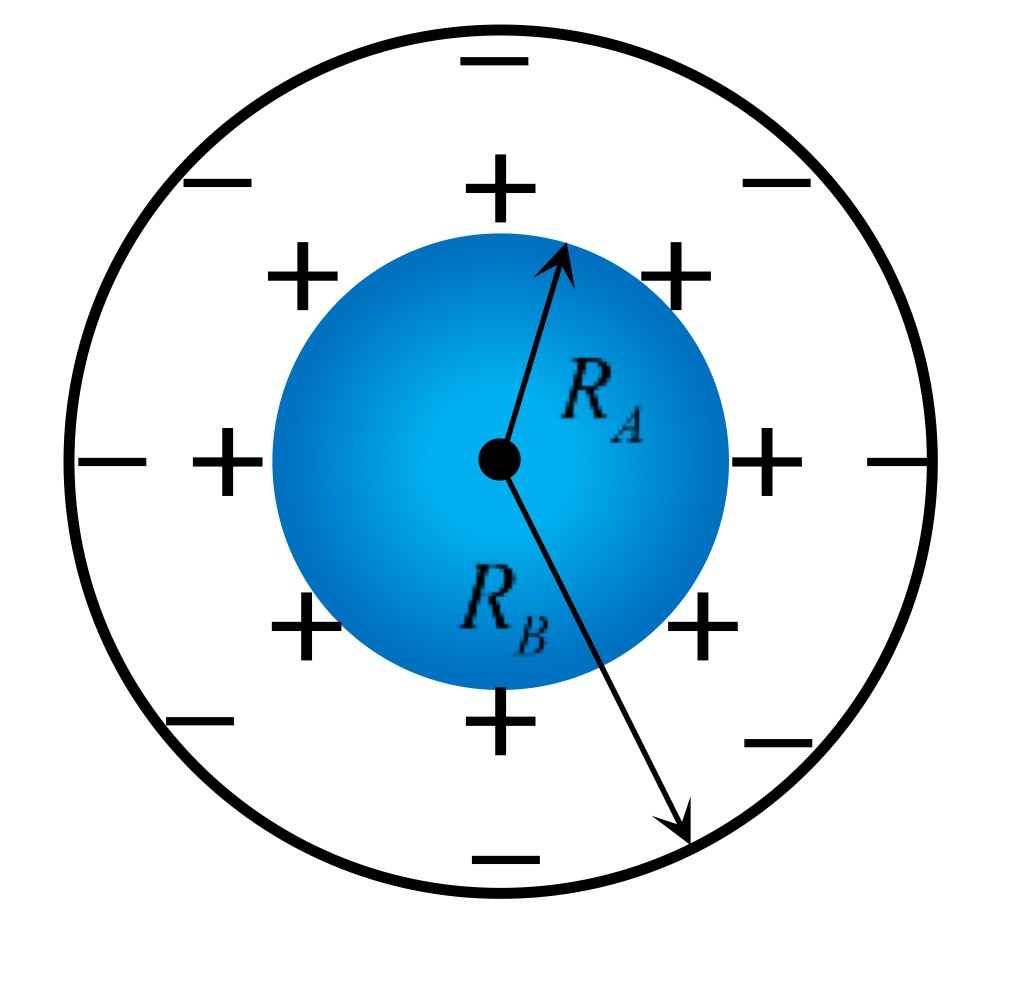
\includegraphics[width=0.18\linewidth]{image/IMG_0422(20231118-140244)}
	\caption{}
	\label{fig:img042220231118-140244}
\end{figure}
		\end{example}
		\begin{solution}
			1.设电量:设内外表面电量分别为$+q,-q$
			
			2.求场强:有结论$E=\frac{q}{4\pi \varepsilon_{0}r^{2}}$
			
			3.算电势差:$U_{ab}=\int\limits_{R_A}^{R_B}{\overrightarrow{E\cdot }d\overrightarrow{r}}=\frac{q}{4\pi \varepsilon _0}\left( \frac{1}{R_A}-\frac{1}{R_B} \right) $
			
			4.套定义
			$C=\frac{q}{U}=4\pi \varepsilon _0\frac{R_AR_B}{R_B-R_A}$
		\end{solution}
		\begin{example}
			求内半径为$R_{A}$,外半径为$R_{B}$,长度为$l$的圆柱体电容器的电容
\begin{figure}[H]
	\centering
	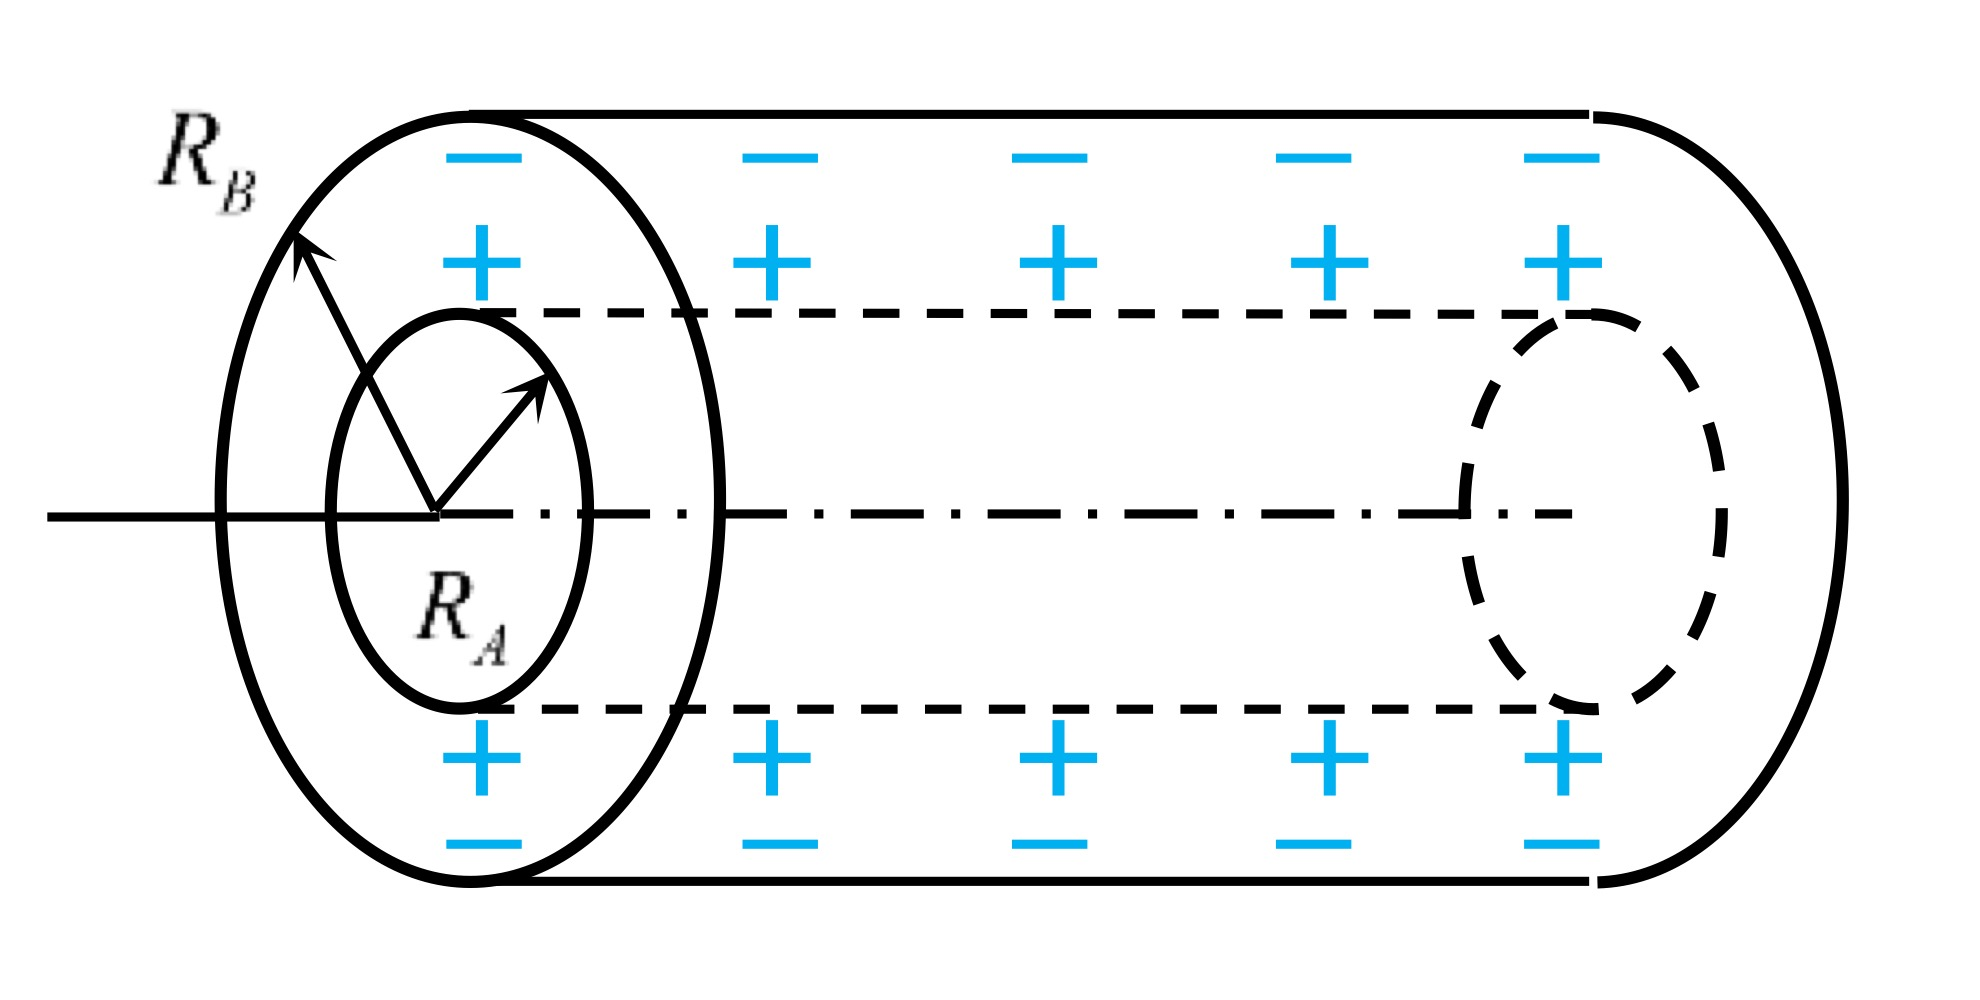
\includegraphics[width=0.18\linewidth]{image/IMG_0421(20231118-140235)}
	\caption{}
	\label{fig:img042120231118-140235}
\end{figure}
		\end{example}
		\begin{solution}
			1.设电量:设内外表面电量分别为$+q,-q$
			
			2.求场强:有结论$E=\frac{\lambda}{2\pi\varepsilon_{0}r}$
			
			3.算电势差$U_{ab}=\int\limits_{R_A}^{R_B}{\overrightarrow{E\cdot }d\overrightarrow{r}}=\frac{q}{2\pi \varepsilon _0l}\ln \frac{R_B}{R_A}$
			
			4.套定义$C=\frac{q}{U}=C=\frac{2\pi \varepsilon _0l}{\ln \frac{R_B}{R_A}}$
		\end{solution}
		\section{电场能}
		\begin{introduction}
			\item 电场能密度
			\item 电场能
		\end{introduction}
		\subsection{\color{red}\text{电场能密度}}
		\begin{definition}
			我们定义电场能密度为
			\begin{equation*}
				w_{e}=\frac{1}{2}\varepsilon_{0}\varepsilon_{r}E^{2}
			\end{equation*}
		\end{definition}
		\subsection{\color{red}\text{电场能}}
		\begin{definition}
			我们定义电场能为
			\begin{equation*}
				W=\frac{Q^{2}}{2C}=\frac{1}{2}C(U_{1}-U_{2})^{2}=\frac{1}{2}Q(U_{1}-U_{2})=\iiint{\frac{1}{2}\varepsilon _0\varepsilon _rE^2dV}
			\end{equation*}
		\end{definition}
		下面这一题,务必要会分析
		\begin{example}
			平行板电容器真空时,各个状态$\sigma_{0},E_{0},U_{0},D_{0},C_{0},W_{e_{0}} $
			
			求:1.充电后断开电源,插入$\varepsilon_{r}$的介质
			
			2.充电后保持电压不变,插入$\varepsilon_{r}$的介质;
			
			这两种情况下的$\sigma,E,U,D,C,W_{e} $
		\end{example}
		\begin{solution}
			1.断开电源后,没有放电,两极板上电量不变,于是$\sigma=\sigma_{0}$
			
			介质中场强$E=\frac{E_{0}}{\varepsilon_{r}}$
			
			电势差$U=Ed=\frac{U_{0}}{\varepsilon_{r}}$
			
			电位移矢量:真空时,$D_{0}=\sigma_{0}$
			
			插入介质后$D=\varepsilon_{0}\varepsilon_{r}E=\varepsilon_{0}E_{0}=\sigma_{0}=D_{0}$
			
			电容$C=\varepsilon_{r}C$
			
			能量$W_{e}=\frac{q^{2}}{2C}$,故$W_{e}=\frac{W_{e_{0}}}{\varepsilon_{r}}$
			
			2.
			电压不变,显然场强也不变
			
			电荷面密度:$\frac{\sigma _0}{\varepsilon _0}=\frac{\sigma}{\varepsilon _0\varepsilon _r}\rightarrow \sigma =\varepsilon _r\sigma _0$
			
			电位移矢量:$D=\sigma =\varepsilon _r\sigma _0=\varepsilon _rD_0$
			
			电容$C=\varepsilon_{r}C$
			
			电容器能量:$W_e=\frac{1}{2}qU=\frac{1}{2}\varepsilon _rq_0U=\varepsilon _rW_{e_0}$
		\end{solution}
		\section{习题训练}
		\begin{exercise}
			如图,二无限大均匀带电平面,平行放置,面密度分别为$\sigma$和 2$\sigma$,则二平面间的电场强度大小$E =?$;$A$板单位面积所受的电场力大小为$?$。
\begin{figure}[H]
	\centering
	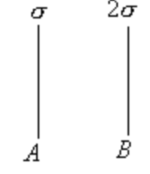
\includegraphics[width=0.1\linewidth]{image/图片1}
	\caption{}
	\label{fig:1}
\end{figure}
		\end{exercise}
		\begin{solution}
			内容...
		\end{solution}
		\begin{exercise}
			如图, 将一均匀带电为$+Q$的细塑料棒弯成半径为$R$的圆弧,圆弧的缺口长度为$d ( d<<R)$,则圆心$O$处场强的大小$E=?$;电场的方向为$?$。
\begin{figure}[H]
	\centering
	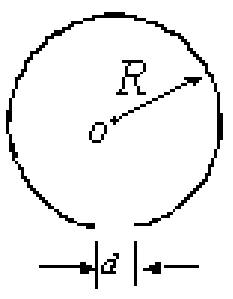
\includegraphics[width=0.1\linewidth]{image/图片2}
	\caption{}
	\label{fig:2}
\end{figure}
		\end{exercise}
		\begin{solution}
			内容...
		\end{solution}
		\begin{exercise}
			一点电荷$q$位于一立方体中心,立方体边长为$a$。则通过立方体一个面的电通量$\varphi$ =?;如果将这个电荷移到立方体的一个顶点$O$上,这时通过立方体BDFE面的电通量$\varphi$ =?			
\begin{figure}[H]
	\centering
	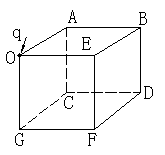
\includegraphics[width=0.1\linewidth]{image/图片3}
	\caption{}
	\label{fig:3}
\end{figure}
		\end{exercise}
		\begin{solution}
			内容...
		\end{solution}
		\begin{exercise}
			选无限远处为电势零点,已知半径为$R$的导体球带电后的电势为$U_{0}$,则球外离球心距离为$r$处的电势为$U=?$;电场强度的大小$E=?$
		\end{exercise}
		\begin{solution}
			内容...
		\end{solution}
		\begin{exercise}
			边长为$a$的正方形的三个顶点上固定的三个点电荷如图所示。以无穷远为零电势点,则$C$点电势$U_{C} =?$;今将一电量为$+q$的点电荷从$C$点移到无穷远,则电场力对该电荷做功$A=?$
\begin{figure}[H]
	\centering
	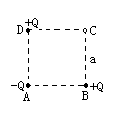
\includegraphics[width=0.1\linewidth]{image/图片4}
	\caption{}
	\label{fig:4}
\end{figure}
		\end{exercise}
		\begin{solution}
			内容...
		\end{solution}
		\begin{exercise}
			半径为$R$的导体球,带有电荷$q$,球外有一内外半径分别为$2R$和$3R$的同心导体球壳,球壳上带有电荷 $2q$,以无穷远处为电势零点,则内球的电势$U_{1}$=? ;外壳的电势$U_{2}$=?
\begin{figure}[H]
	\centering
	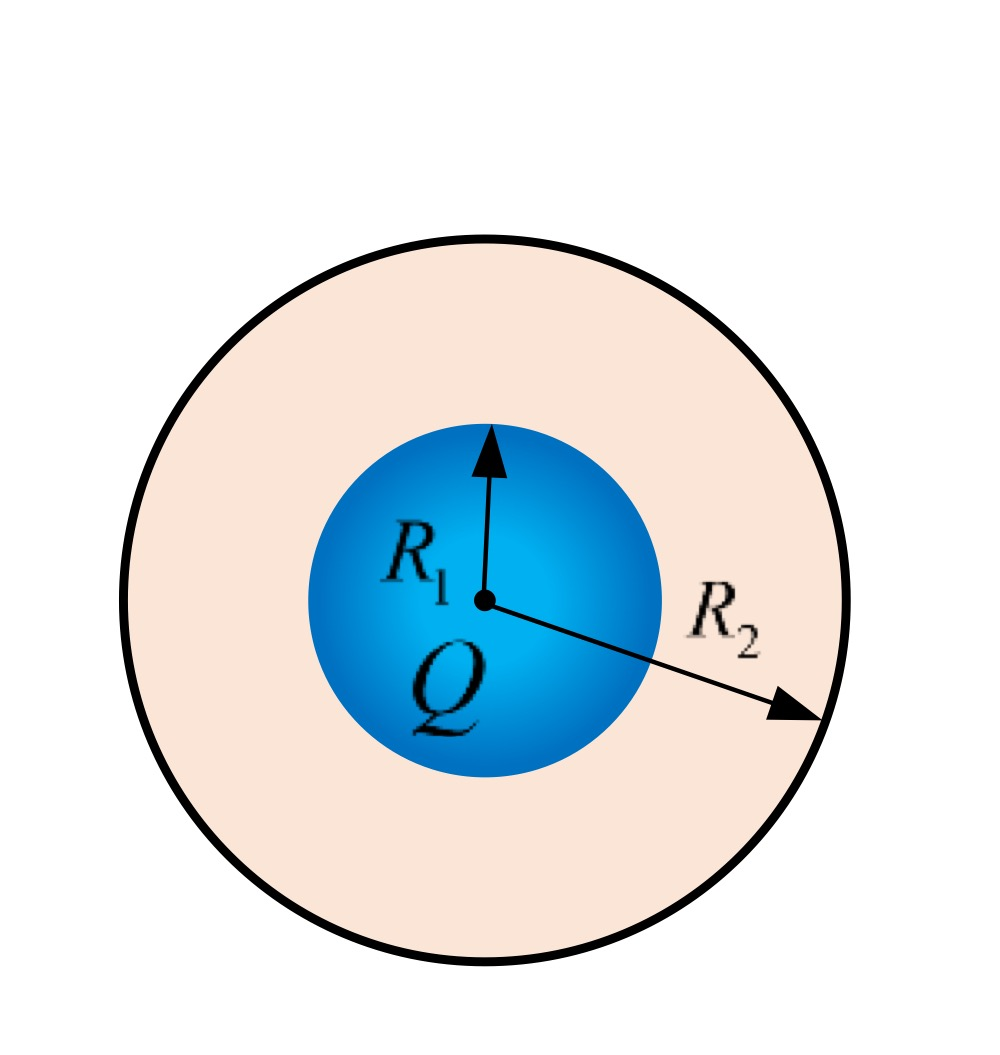
\includegraphics[width=0.1\linewidth]{image/IMG_0418(20231118-125659)}
	\caption{}
	\label{fig:img041820231118-125659}
\end{figure}
		\end{exercise}
		\begin{solution}
			内容...
		\end{solution}
		\begin{exercise}
			空气平行板电容器,接上电源后,两极板上的电荷面密度分别为$\pm \sigma_{0}$。在保持电源接通情况下,将相对介电常数为$\varepsilon_{r}$的各向同性均匀电介质充满其中,忽略边缘效应,介质中的场强大小为?;如果断开电源后再充介质,则介质中的场强大小为?。
		\end{exercise}
		\begin{solution}
			内容...
		\end{solution}
		\begin{exercise}
			平行板电容器两极板间距为$d$,将它充电至电势差为$U_{0}$,然后断开电源,插入厚度为$\frac{d}{2}$、相对介电常数为$\varepsilon_{r}$的各向同性均匀介质板,则介质中的电场强度$E =?$,两极板间的电势差$U =?$			
\begin{figure}[H]
	\centering
	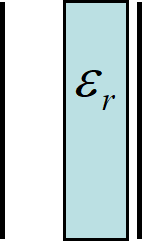
\includegraphics[width=0.1\linewidth]{image/图片6}
	\caption{}
	\label{fig:6}
\end{figure}
		\end{exercise}
		\begin{solution}
		
		\end{solution}
		\begin{exercise}
				半径为$R$的均匀带电金属球体,总电量为$+Q$,将之放置于介电常数为$\varepsilon_{r}$的均匀电介质中,则介质中距球心$r$处$P$点($r>R$)电位移矢量大小$D$ =?,该处电场能量密度$w_{e}= ?$
		\end{exercise}
		\begin{solution}
			内容...
		\end{solution}
		\begin{exercise}
			在真空中有半径分别为$R$和$2R$的两个同心球面,其上分别均匀地带有电量$+Q$和-$3Q$,今将一电量为$+q$的带电粒子从内球面处由静止释放,则该粒子到达外球面时的动能为
\begin{figure}[H]
	\centering
	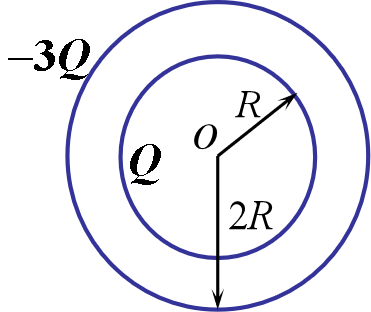
\includegraphics[width=0.1\linewidth]{image/图片7}
	\caption{}
	\label{fig:7}
\end{figure}
		\end{exercise}
		\begin{solution}
			内容...
		\end{solution}
		\begin{exercise}
			如图所示,CDEF为一矩形,边长分别为 $a$和$2a$ ,A点在DC延长线上,CA=$a$。A点有一点电荷$+q$,在CF的中点B点有一点电荷$-q$。若使单位正电荷从C点沿CDEF路径运动到F点,则电场力所做的功A= ? 
\begin{figure}[H]
	\centering
	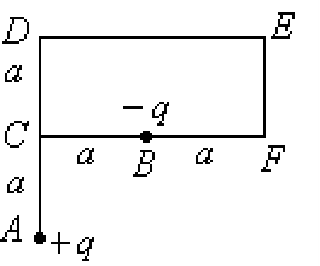
\includegraphics[width=0.15\linewidth]{image/图片8}
	\caption{}
	\label{fig:8}
\end{figure}     
		\end{exercise}
		\begin{solution}
			内容...
		\end{solution}
		\begin{exercise}
			半径分别为$R$和$r$的两个金属球,相距很远。用一根长导线将两球连接,并使它们带电。在忽略导线影响的情况下,两球表面的电荷面密度之比$\frac{\sigma_{R}}{\sigma_{r}}$ 为 ?
		\end{exercise}
		\begin{solution}
			内容...
		\end{solution}
		\begin{exercise}
			一平行板空气电容器,极板面积$S$,间距$d$,充电至带电$Q$后与电源断开,然后用外力缓缓地把极板间距离拉开到$2d$。电容器电场能量改变量为,在此过程中外力所做的功为?
		\end{exercise}
		\begin{solution}
			内容...
		\end{solution}
		\begin{exercise}
			一“无限长”均匀带电直线,电荷线密度为 ,则它在与直线相距为$r$的P处产生的电场强度大小$E=?$;在该电场作用下,一个质量为$m$、带电量为$-q$的质点以直线为轴线作匀速率圆周运动,该质点的速率$v =$?
		\end{exercise}
		\begin{solution}
			内容...
		\end{solution}
		\begin{exercise}
			A和B为真空中两块平行无限大带电平面,已知两平面间的电场强度大小为$E_{0}$,两平面外侧的电场强度大小都是$\frac{E_{0}}{3}$,电场方向如图所示,则A、B两平面的电荷面密度分别为多少			
\begin{figure}[H]
	\centering
	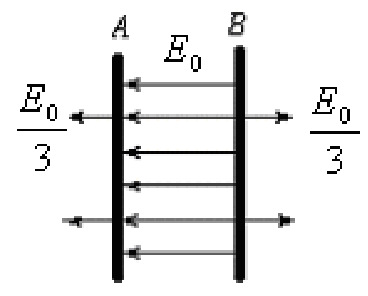
\includegraphics[width=0.1\linewidth]{image/图片9}
	\caption{}
	\label{fig:9}
\end{figure}
		\end{exercise}
		\begin{solution}
			内容...
		\end{solution}
		\begin{exercise}
			边长为$a$的正方形四个顶角上各有一点电荷$q$,则其中垂线上与中心相距为$a$的$P$点的电场强度大小为?
		\end{exercise}
		\begin{solution}
			内容...
		\end{solution}
		\begin{exercise}
		真空中两平行的均匀带电平板相距为$d$,面积为$S$,且有$d'<<S$,带电量分别为$+q$与$-q$,则两板间的作用力大小为
		\end{exercise}
		\begin{solution}
			内容...
		\end{solution}
		\begin{exercise}
			一个细而长的圆柱面上有一条平行于轴线的窄缝,窄缝的宽度$l$远小于圆柱半径,如图所示轴线中点О点的场强大小=?、方向?若取O点为电势零点,则在轴线与窄缝之间离轴线$\frac{R}{3}$处P点的电势?
		\end{exercise}
		\begin{solution}
			内容...
		\end{solution}
		\begin{exercise}
			如图所示,一个均匀带电球层,电量为$Q$,球层内表面半径为$R_{1}$、外表面半径为$R_{2}$,以无穷远处为电势零点,求空腔内任意一点的电势
\begin{figure}[H]
	\centering
	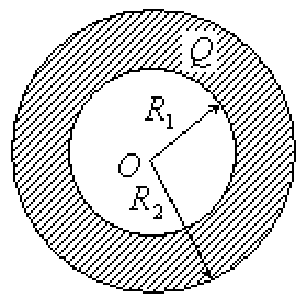
\includegraphics[width=0.15\linewidth]{image/图片10}
	\caption{}
	\label{fig:10}
\end{figure}
		\end{exercise}
		\begin{solution}
			内容...
		\end{solution}
		\begin{exercise}
			一无限长均匀带电圆柱体,体电荷密度为$\rho$,截面半径为$R$。
			
			(1)求柱内外电场强度分布;
			
			(2)以轴线处为电势零点,求柱内外的电势分布。
		\end{exercise}
		\begin{solution}
			内容...
		\end{solution}
		\begin{exercise}
			二金属球壳同心放置,内金属球壳半径为$R_{1}$,外金属球壳半径为$R_{2}$,中间充以介电常数为$\varepsilon_{r}$的均匀电介质。已知二金属球壳电势差为$U_{0}$,且内球壳电势比外球壳高。求:
			
			(1)内球壳的带电量$Q$。
			
			(2)二球壳之间的电场能量
		\end{exercise}
		\begin{solution}
			内容...
		\end{solution}
		\begin{exercise}
			为了测量电介质材料的相对介电常数,将一块厚为 $1.5cm$ 的平板材料慢慢地
			插进一电容器的距离为 $2.0cm$ 的两平行板之间。在插入过程中,电容器的电荷保
			持不变。插入之后,两板间的电势差减少为原来的 $60\%$ ,求电介
			质的相对介电常数多大?
		\end{exercise}
		\begin{solution}
			内容...
		\end{solution}
		\begin{exercise}
			两块导体平板,面积为 S,分别带电荷$q_{1}$和 $q_{2}$,两极板间距远小于平板的线
			度。求平板各表面的电荷密度。
		\end{exercise}
		\begin{solution}
			内容...
		\end{solution}
		\begin{exercise}
			一带电圆环,电荷线密度分布为$\lambda =\lambda_{0}\cos^{2}\theta$,求环心处的电势

		\end{exercise}
	\chapter{磁学}
	\section{磁感应强度}
	\begin{introduction}
		\item 毕奥萨伐尔定律(重要)
		\item 安培环路定理(重要)
	\end{introduction}
	\subsection{\color{red}\text{毕奥萨伐尔定律}}
	\begin{theorem}[毕奥萨伐尔定律]
		\begin{equation*}
			dB=\frac{\mu _0}{4\pi}\frac{Id\overrightarrow{l}\times \overrightarrow{\hat{r}}}{r^2}\left( r\text{的方向:从电流源所在位置指向场点} \right) 
		\end{equation*}
	\end{theorem}
	\begin{remark}
		真空磁导率:$\mu _0=4\pi\times 10^{-7}$
	\end{remark}
	\subsection{\color{red}\text{安培环路定理}}
	\begin{theorem}
		\begin{equation*}
			\ointctrclockwise_L{\overrightarrow{B}\cdot d\overrightarrow{l}}=\mu _0\sum_{L\text{内}}{I}
		\end{equation*}
	\end{theorem}
	\begin{note}
		若利用斯托克斯定理,我们有
		\begin{equation*}
			\ointctrclockwise_L{\overrightarrow{B}\cdot d\overrightarrow{l}}=\mu _0\sum_{L\text{内}}{I}\rightarrow \iint_S{\left( \nabla \times \overrightarrow{B} \right) \cdot d\overrightarrow{S}}=\mu _0\iint_S{j\cdot d\overrightarrow{S}}
		\end{equation*}
		
		即
		\begin{equation*}
			\left( \nabla \times \overrightarrow{B} \right) =\mu _0\overrightarrow{j}
		\end{equation*}
		
		说明$B$的旋度不为零,说明为有旋场,即磁场为闭合曲线
	\end{note}
	\begin{remark}
		环路定理直于环路内电流有关,与电流位置以及环路外电流无关
	\end{remark}
	\begin{remark}
		$\sum_{L\text{内}}{I}$是环路内的净电流(所有电流的代数和)
	\end{remark}
	\begin{remark}
		环路上的磁感应强度$B$,不仅受环路内电流影响,还受环路外电流影响
	\end{remark}
	\subsection{常见的导体磁感应强度总结}
	\begin{example}
		一段有限长$L$载流直导线,通有电流为$I$,求距离$a$处的$P$点磁感应强度
\begin{figure}[H]
	\centering
	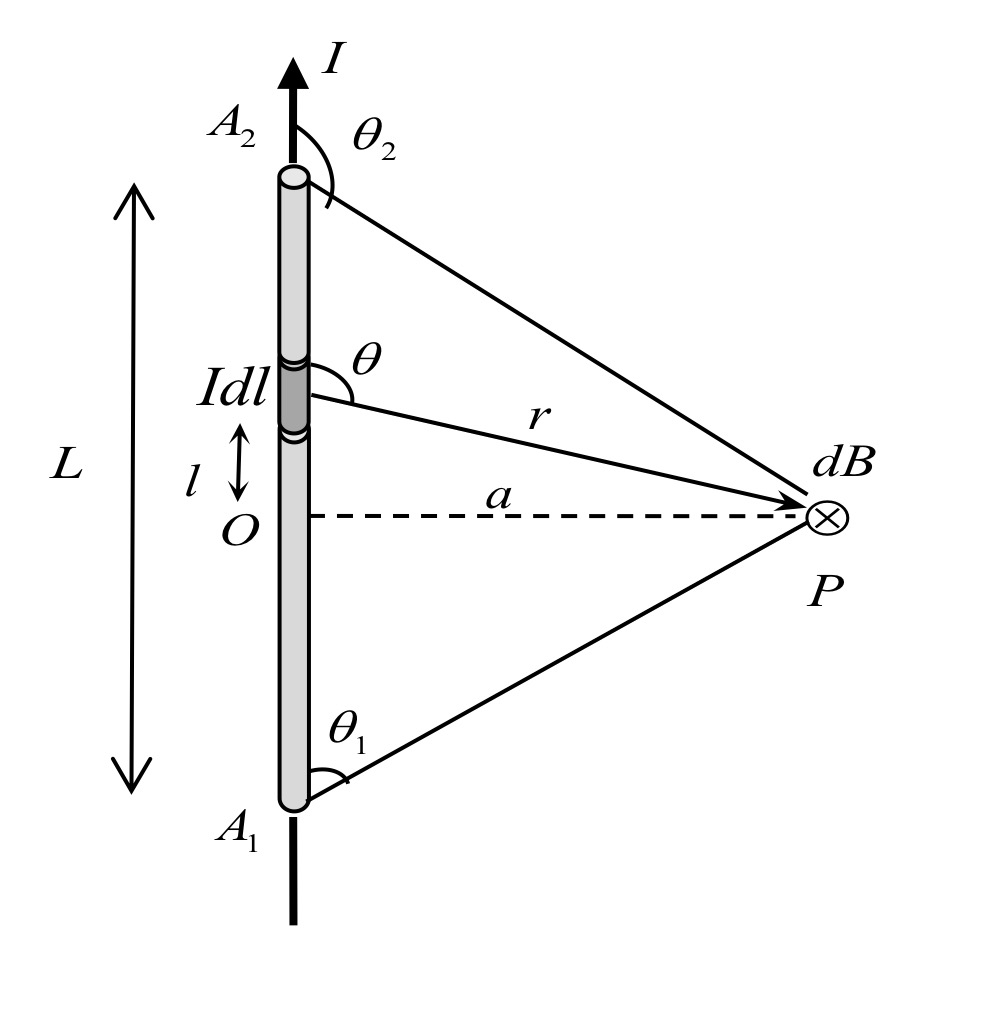
\includegraphics[width=0.18\linewidth]{image/IMG_0425(20231121-204507)}
	\caption{}
	\label{fig:img042520231121-204507}
\end{figure}
	\end{example}
	\begin{solution}
		我们取任一电流源$Idl$,此时在$P$点产生的磁感应大小为
		\begin{equation*}
			dB=\frac{\mu _0}{4\pi}\frac{Idl\sin \theta}{r^2}
		\end{equation*}
		
		又因为$r=\mathrm{a}\csc \theta ,l=\mathrm{a}\cot \theta ,dl=\mathrm{a}\csc ^2\theta d\theta $
		
		积分可得
		\begin{equation*}
			B=\frac{\mu _0 I}{4\pi a}\left( \cos \theta _1-\cos \theta _2 \right)
		\end{equation*}
	\end{solution}
	\begin{note}
		此时若导线长度为无限长,则
		\begin{equation*}
			B=\frac{\mu _0 I}{2\pi a}
		\end{equation*}
	\end{note}
	\begin{remark}
		有了这个公式,我们可以求平板电流,不论是有限大还是无限大的,此外,一些圆弧体电流也可求得
	\end{remark}
	\begin{example}
		设螺线管半径为$a$,扎线密度为$ n$,电流为$I$,求轴线上$O$点处的磁感应强度
		\begin{figure}[H]
	\centering
	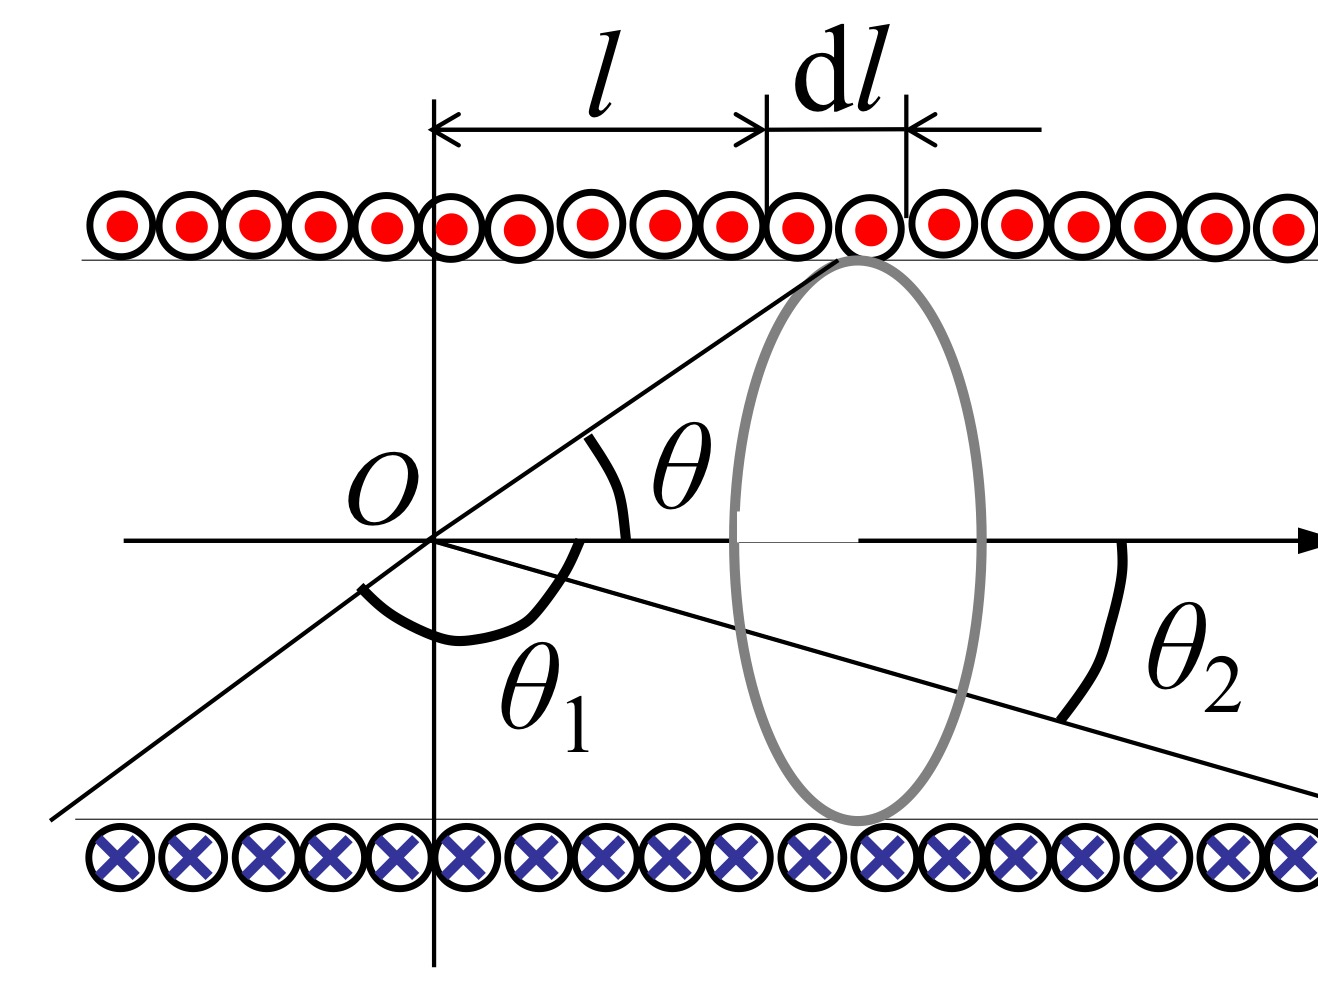
\includegraphics[width=0.18\linewidth]{image/IMG_0426(20231121-204759)}
	\caption{}
	\label{fig:img042620231121-204759}
\end{figure}
	\end{example}
	\begin{solution}
		这里我们要用到一个结论:
		
		单位圆环对$O$点的磁感应强度为
		\begin{equation*}
			dB=\frac{\mu _0R^2dI}{2\left( x^2+R^2 \right) ^{\frac{3}{2}}}
		\end{equation*}
		
		单位电流为$nI$
		带入对应式子里,我们有
		\begin{equation*}
			dB=\frac{\mu _0a^2nIdl}{2\left( a^2+R^2 \right) ^{\frac{3}{2}}}
		\end{equation*}
		
		又因为$\sin \theta =\frac{a}{\sqrt{a^2+l^2}}\text{和}l=\mathrm{a}\cot \theta \rightarrow dl=-\frac{a}{\sin ^2\theta}d\theta$
		
		我们有
		\begin{equation*}
			dB=-\frac{\mu _0 nI}{2}\sin \theta d\theta 
		\end{equation*}
		
		积分得
		\begin{equation*}
			B=\frac{\mu _0nI}{2}\left( \cos \theta _2-\cos \theta _1 \right) 
		\end{equation*}
	\end{solution}
	\begin{note}
		在管子无穷长的时候,我们能得到
		\begin{equation*}
				B=\mu _0nI
		\end{equation*}
	\end{note}
	\begin{example}
		设螺绕环半径为$R$(忽略管内半径),扎数为$ N$,电流为$I$,求轴线上$O$点处的磁感应强度
		
\begin{figure}[H]
	\centering
	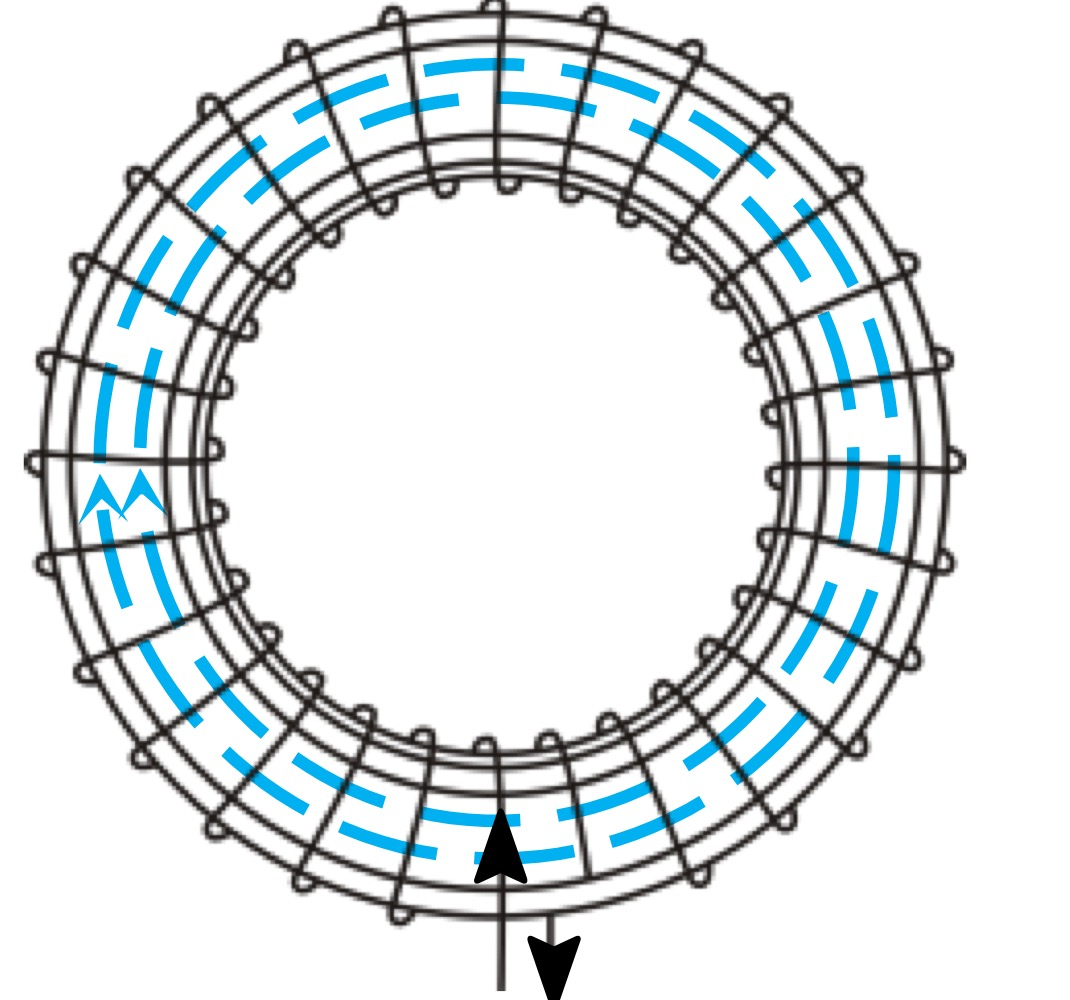
\includegraphics[width=0.18\linewidth]{image/IMG_0427(20231121-205357)}
	\caption{}
	\label{fig:img042720231121-205357}
\end{figure}
	\end{example}
	\begin{solution}
		对于环,我们有环路定理
		\begin{equation*}
			\ointclockwise_L{\overrightarrow{B}\cdot dl}=\mu _0NI
		\end{equation*}
		
		解得
		\begin{equation*}
			B=\frac{\mu _0NI}{2\pi r}
		\end{equation*}
	\end{solution}
	\begin{note}
		当$R<<r$,$B=\frac{\mu _0NI}{2\pi r}=\mu _0 nI$,同无限长螺线管
	\end{note}
	\section{磁通量的高斯定理}
	\begin{introduction}
		\item 磁通量(重要)
		\item 高斯定理(重要)
		\item 磁矢势(重要)
	\end{introduction}
	\subsection{\color{red}\text{磁通量}}
	\begin{definition}[磁通量]
		我们定义穿过单位面积的磁场线条数为通量,即
		\begin{equation*}
			d\varPhi =\overrightarrow{B}\cdot d\overrightarrow{S}\Rrightarrow \varPhi =\iint_S{\overrightarrow{B}\cdot d\overrightarrow{S}}
		\end{equation*}
	\end{definition}
	\begin{remark}
		这里面积的方向定义为面法线的方向
	\end{remark}
	\begin{remark}
		对于曲面,向外穿出为正向内穿入为负
	\end{remark}
	\begin{example}
		如图,一无限长直导线通以电流$I$,若有一矩形导体线框与直导线共面且距导线为$a$,试求通过矩形导体线框的磁通量
		
\begin{figure}[H]
	\centering
	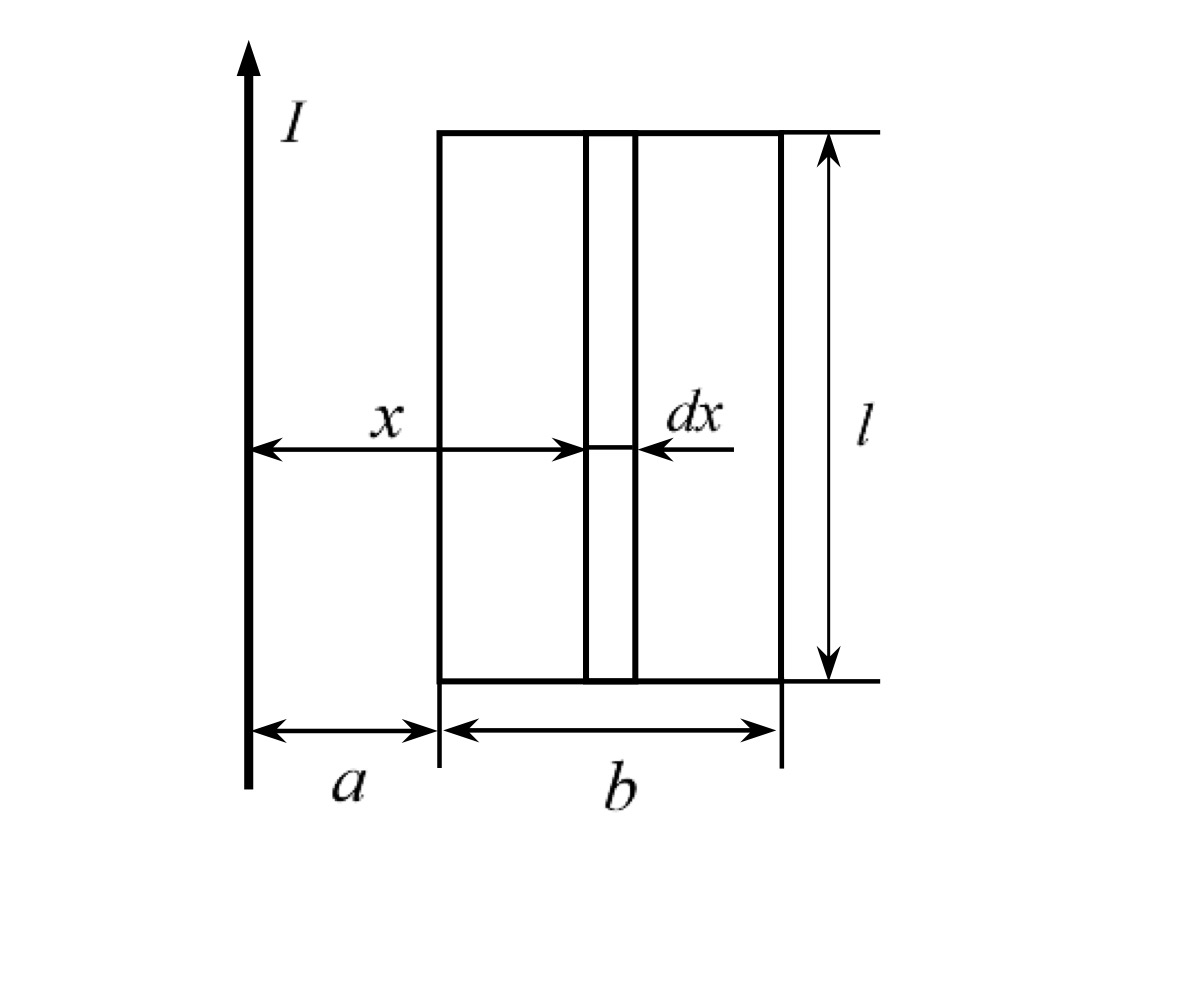
\includegraphics[width=0.18\linewidth]{image/IMG_0429(20231122-122542)}
	\caption{}
	\label{fig:img042920231122-122542}
\end{figure}
	\end{example}
	\begin{solution}
		我们取$dx$的细条,其面积为$ldx$
		
		在此处的磁感应强度为$\frac{\mu _0I}{2\pi x}$,于是我们有
		
		\begin{equation*}
			\varPhi =\iint_S{\overrightarrow{B}\cdot d\overrightarrow{S}}=\frac{\mu _0Il}{2\pi}\ln \frac{a+b}{a}
		\end{equation*}
	\end{solution}
	\subsection{\color{red}\text{高斯定理}}
	\begin{theorem}[高斯定理]
		静电场中穿过任一曲面的磁通量等于0,
		
		用公式表示就是
		\begin{equation*}
			\oiint{\overrightarrow{B}\cdot d\overrightarrow{S}}=0
		\end{equation*}
		$V$是闭面$S$所包围的空间
	\end{theorem}
	\begin{note}
		此时我们如果用高斯公式
		\begin{equation*}
			\oiint{\overrightarrow{B}\cdot d\overrightarrow{S}}=\oiiint\limits_V{\nabla \cdot \overrightarrow{B}dV}
		\end{equation*}
		
		可得到
		\begin{equation*}
			\nabla \cdot \overrightarrow{B}=0
		\end{equation*}
		表明恒磁场的散度为0,即恒磁场是无源场
	\end{note}
		\subsection{\color{red}\text{磁矢势}}
		
		\begin{definition}
			效仿电势,我们可以找到一个量$A$,使得其在数学上满足
			\begin{equation*}
				\ointclockwise_L{A\cdot dl}=\iint_S{B\cdot dS}
			\end{equation*}
			
			我们称$A$为磁矢势
		\end{definition}
		
		这种题目,我们通常就按照定义走,先求出通过一个面的磁通量,再用定义即可
		\begin{example}
			一根无限长直导线,载有电流$I$,求其在空间中的磁矢势分布
		\end{example}
		\begin{solution}
			如图,取一个闭合回路
			
\begin{figure}[H]
	\centering
	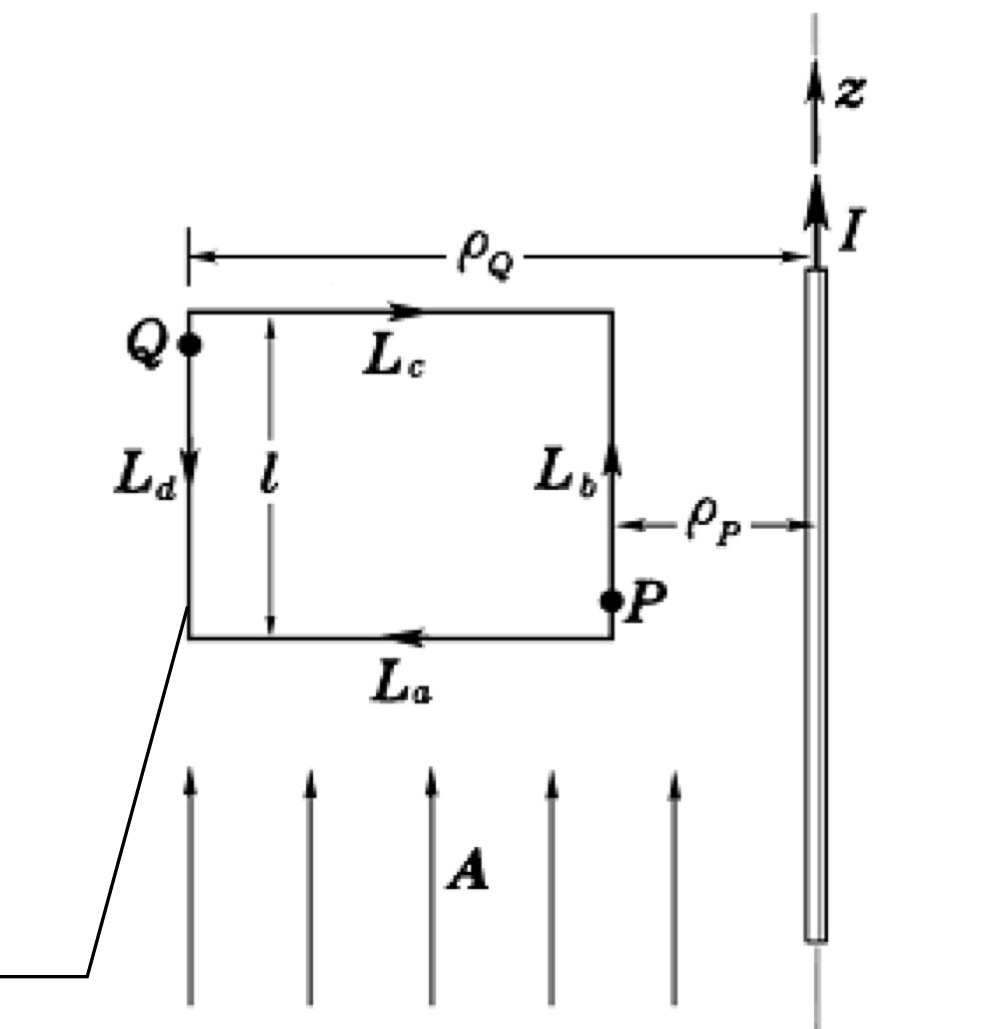
\includegraphics[width=0.18\linewidth]{image/IMG_0431(20231122-125850)}
	\caption{}
	\label{fig:img043120231122-125850}
\end{figure}
		\end{solution}
		\begin{example}
			无限长圆柱形导体,半径为$R$,载有带界面上均匀分布的电流$I$,求磁矢势
		\end{example}
		\begin{example}
			
			$r<R$,时,如图
			
\begin{figure}[H]
	\centering
	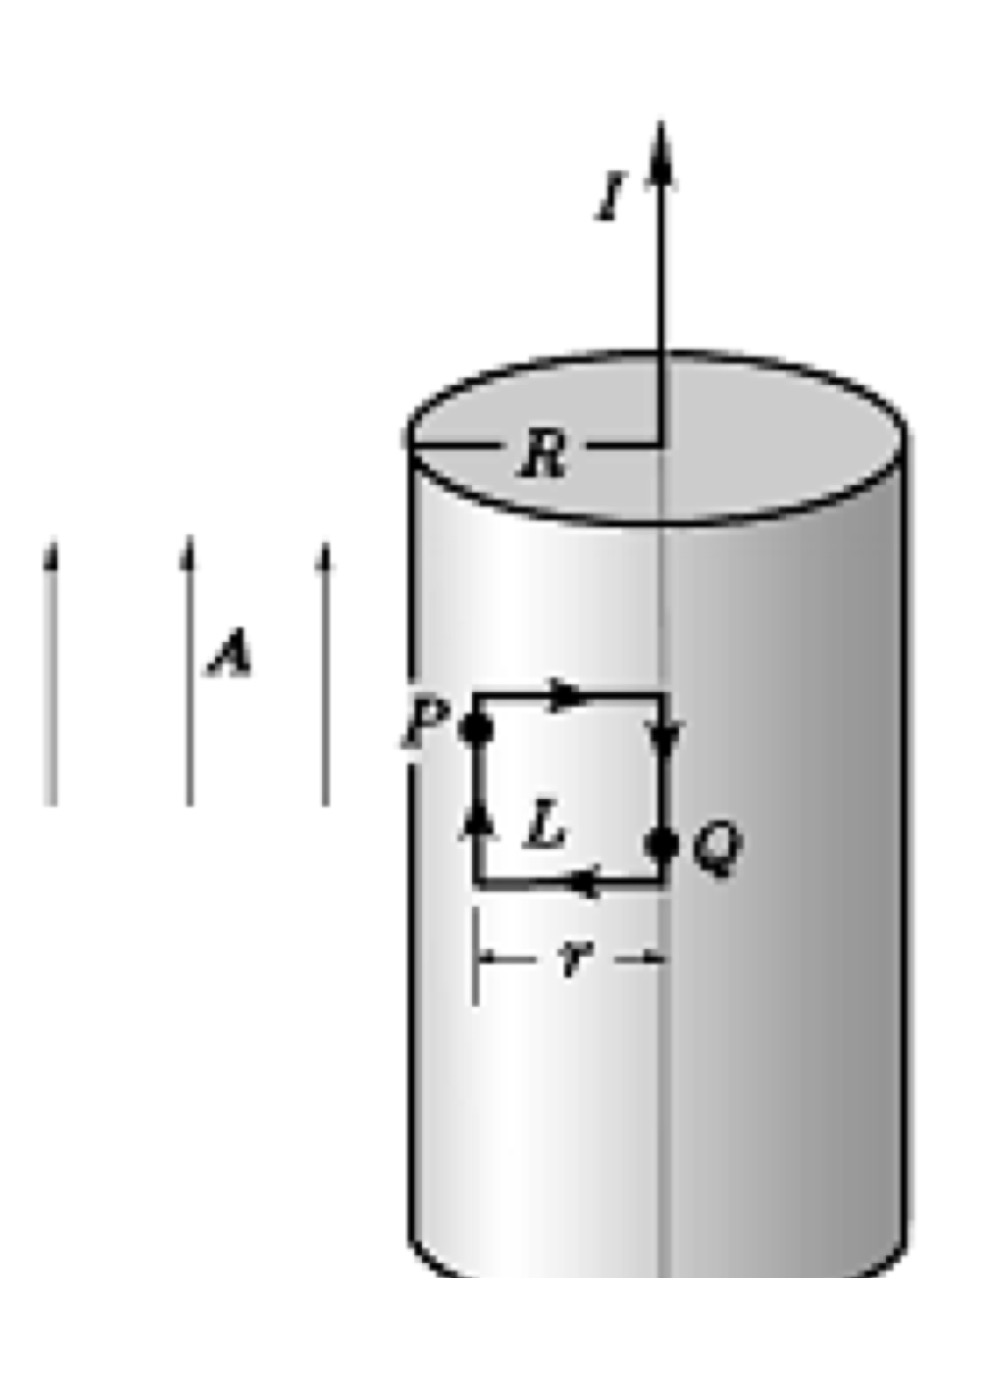
\includegraphics[width=0.18\linewidth]{image/IMG_0432(20231122-130153)}
	\caption{}
	\label{fig:img043220231122-130153}
\end{figure}
			
			
			$r>R$,时,如图
			
\begin{figure}[H]
	\centering
	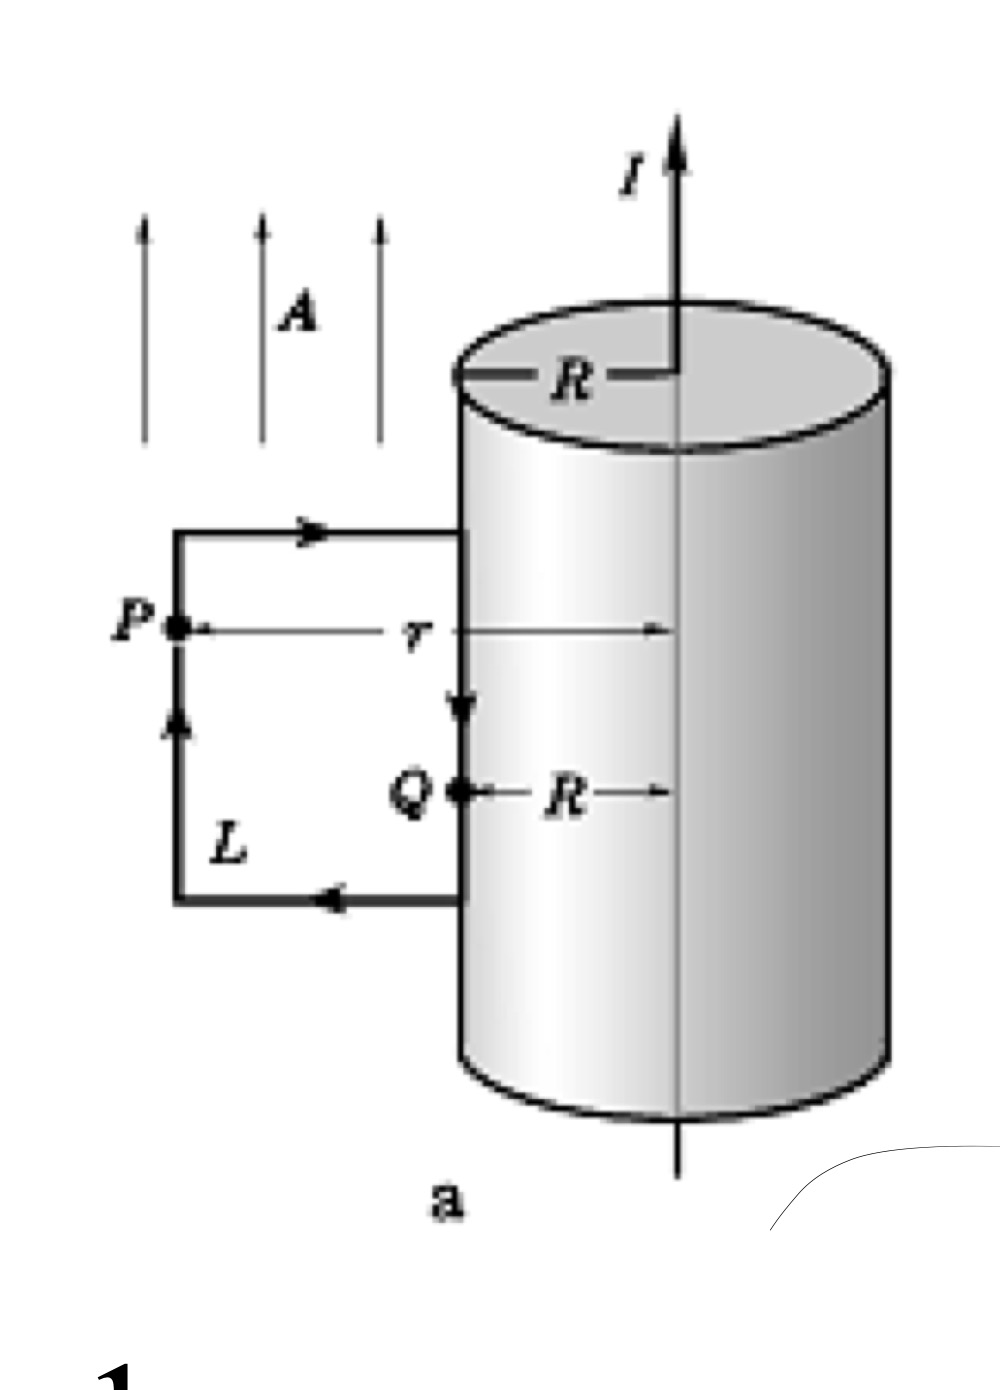
\includegraphics[width=0.18\linewidth]{image/IMG_0433(20231122-130208)}
	\caption{}
	\label{fig:img043320231122-130208}
\end{figure}
			
			
		\end{example}
		\begin{example}
			一对同轴无穷长直的空心导体圆筒,内、外筒半径分别为$R_{1}$和$R_{2}$(筒壁厚度可以忽略)。电流$I$沿
			内筒流去,沿外筒流回(见本题图),
			
			(1)计算两筒间的磁感应强度$B$;
			
			(2)通过长度为$L$的一段截面(图中阴影区)的磁通量;
			
			(3)计算磁矢势A在两筒间的分布
			
			
\begin{figure}[H]
	\centering
	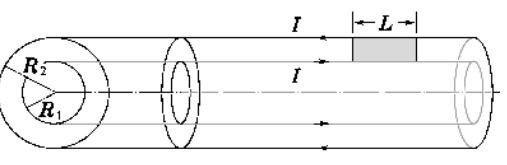
\includegraphics[width=0.18\linewidth]{image/1700629154615}
	\caption{}
	\label{fig:1700629154615}
\end{figure}
		\end{example}
	\section{磁场对载流导线的作用}
	\begin{introduction}
		\item 安培力(重要)
		\item 磁矩(重要)
		\item 磁力矩(重要)
	\end{introduction}
	\subsection{\color{red}\text{安培力}}
	这一部分,我们只需要进行记忆安培力的公式
	\begin{equation*}
		\overrightarrow{F}=\int{I\cdot \overrightarrow{dl}\times \overrightarrow{B}}
	\end{equation*}
	剩下的就是高中题目的难度了
	
	\begin{remark}
		$	\overrightarrow{F}$的方向用右手定则判断,就是矢量叉乘的大拇指方向
	\end{remark}
	\subsection{\color{red}\text{磁矩}}
	我们如下定义磁矩
	\begin{definition}[磁矩]
		\begin{equation*}
			\overrightarrow{m}=NIS
		\end{equation*}		
	\end{definition}
	\begin{remark}
		此时磁矩的方向可用右手定则判断:电流沿着四指,大拇指朝向就是磁矩的方向
	\end{remark}
		\subsection{\color{red}\text{磁力矩}}
		我们如下定义磁力矩
		\begin{definition}[磁矩]
			\begin{equation}
				\overrightarrow{M}=\overrightarrow{m}\times \overrightarrow{B}
			\end{equation}		
		\end{definition}
		
		这一部分的习题不算特别难,不单独出现,往往结合起来考,我们在习题训练里面写
	\section{带电粒子在磁场中的运动}
	\begin{introduction}
		\item 洛伦兹力(重要)
	\end{introduction}
	\subsection{\color{red}\text{洛伦兹力}}
	这一部分的内容,高中生来了都会写,我们回顾一下公式,也顺便回顾一下我们那逝去的青春
	
	洛伦兹力公式
	\begin{equation*}
		\overrightarrow{f}=q\overrightarrow{v}\times \overrightarrow{B}
	\end{equation*}
	
	半径公式
	\begin{equation*}
		R=\frac{mv}{Bq}
	\end{equation*}
	
	周期公式
	\begin{equation*}
		T=\frac{2\pi R}{v}=\frac{2\pi m}{Bq}
	\end{equation*}
	
	其余的东西,如回旋加速器,磁流体发电机,见《恒磁场》ppt 74页到81页
	
	这部分的题目,见习题训练
	\section{磁介质}
	\begin{introduction}
		\item 磁介质(重要)
	\end{introduction}	
	\subsection{\color{red}\text{磁介质}}
	\begin{theorem}[磁介质高斯定理]
		\begin{equation*}
			\oint_L{\overrightarrow{H}\cdot d\overrightarrow{l}}=\sum{I_{\text{内}}}
		\end{equation*}
	\end{theorem}
	\begin{note}
		(1)$H=\frac{B}{\mu _0\mu _r}=\frac{B}{\mu _0}-M\left( M\text{为磁化强度} \right) $
		
		(2)$\text{磁导率}\mu =\mu _0\mu _r\text{,相对磁导率}\mu _r\text{,真空中相对磁导率}\mu _r=1$
		
		(3)此定理不仅适用于含有介质的,还适用于不含有介质的
		
	\end{note}
	\begin{remark}
	$	\mu _r>1$顺磁质
		
		$\mu _r<1$抗磁质
		
		$\mu _r>>1$铁磁质
	\end{remark}
	\begin{remark}
		关于磁化强度的知识,请看《磁介质》第1页到19页
	\end{remark}
	
	\section{磁场的功与能}
	\begin{introduction}
		\item 载流导体运动时的功(蛮重要)
		\item 磁场能(重要)
	\end{introduction}
	\subsection{\color{red}\text{载流导体运动时的功}}
	这里的话,给出做的功的统一式子
	\begin{equation*}
		A=\int\limits_{\varPhi _1}^{\varPhi _2}{Id\varPhi}
	\end{equation*}
	
	只需要记住这个即可
	\subsection{\color{red}\text{磁场能}}
	\begin{definition}[能量密度]
		我们定义能量密度为
		\begin{equation*}
			w=\frac{1}{2}BH
		\end{equation*}
	\end{definition}
	\begin{note}
		此时空间站的磁场的表达式为
		\begin{equation*}
			W=\oiiint_V{wdV}
		\end{equation*}
	\end{note}
	这个部分习题见习题训练
	\section{习题训练}
	\begin{exercise}
		如图所示的长导线中通有电流,图中圆心$O$处的磁感应强度的大小为    ?                ,方向 ? 
		
		                           。
\begin{figure}[H]
	\centering
	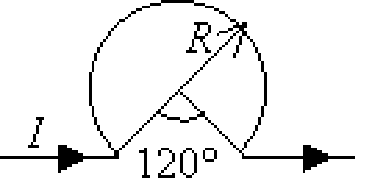
\includegraphics[width=0.18\linewidth]{image/图片11}
	\caption{}
	\label{fig:11}
\end{figure}
	\end{exercise}
	\begin{exercise}
		两根平行放置的无限长载流导线,均通有电流$I_{0}$,电流流向如图所示,则P处磁感应强度值$ B_{P}  $=?,$\oint_L{\overrightarrow{B}\cdot d\overrightarrow{l}}$ =?   
		
\begin{figure}[H]
	\centering
	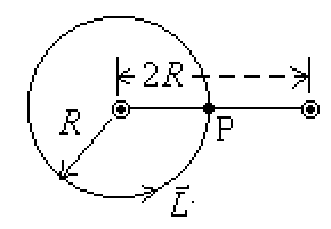
\includegraphics[width=0.18\linewidth]{image/图片12png}
	\caption{}
	\label{fig:12png}
\end{figure}
		            。
	\end{exercise}
	\begin{exercise}
		如图所示,薄中空圆盘的内、外半径分别为$R_{1}$和$R_{2}$,均匀带有电量$+Q_{0}$,可绕通过圆心$O$且垂直盘面的轴线以匀角速度$\omega$转动。求圆盘转动时圆心$O$处的磁感应强度的大小和方向
		
\begin{figure}[H]
	\centering
	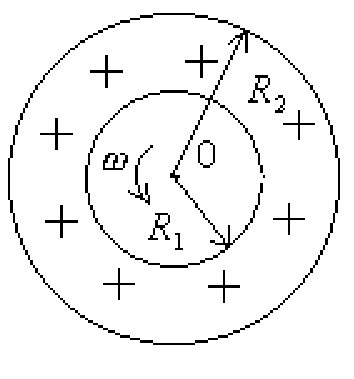
\includegraphics[width=0.18\linewidth]{image/图片13}
	\caption{}
	\label{fig:13}
\end{figure}
	\end{exercise}
	\begin{exercise}
		如图所示,半径为$R$的无限长直圆柱导体,均匀地通有电流 $I_{0}$。求通过图示ABCD平面的磁通量
		
		
\begin{figure}[H]
	\centering
	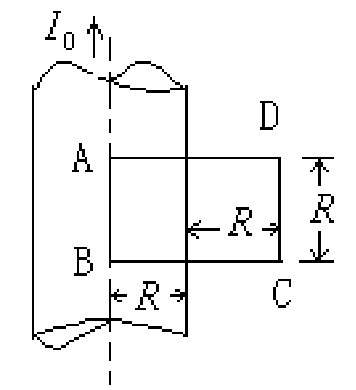
\includegraphics[width=0.18\linewidth]{image/图片14}
	\caption{}
	\label{fig:14}
\end{figure}
	\end{exercise}
	\begin{exercise}
		如图所示,矩形线圈ACDO通有电流$I$,将它置于均匀磁场中,磁场方向与$x$轴正方向一致,线圈平面与$x$轴之间的夹角为 $\alpha$,($\alpha<90\degree$)。若AO边在Oy轴上,且线圈可绕Oy轴自由转动,则线圈的转动方向为=?。
		
\begin{figure}[H]
	\centering
	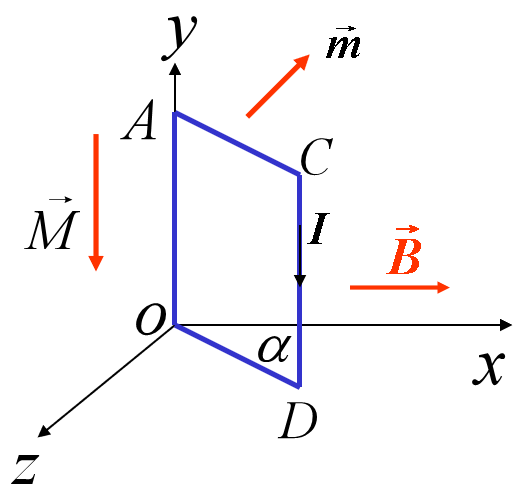
\includegraphics[width=0.18\linewidth]{image/图片15}
	\caption{}
	\label{fig:15}
\end{figure}
		
	\end{exercise}
	\begin{exercise}
		一个质量为$M$、半径为$R$的电介质圆盘均匀地带有电荷,面电荷密度为$\sigma$,圆盘以$\omega$的角速度绕通过盘心且垂直于盘面的轴旋转。
		
		(1)求圆盘的磁矩;
		
		(2)证明圆盘磁矩$m$与角动量$L$的关系为  $\overrightarrow{m}=\frac{q}{2M}\overrightarrow{L}$,其中为圆盘所带的总电量
	\end{exercise}
	\begin{exercise}
		一无限长导线弯成如图所示的形状。其中半圆弧位于Oyz平面内,半径为R,圆心在坐标原点O处。一部分导线与z轴重合,另一部分导线与x轴平行。当导线通有电流$I$时,坐标原点O处的磁感应强度$B $= ?
		
		
\begin{figure}[H]
	\centering
	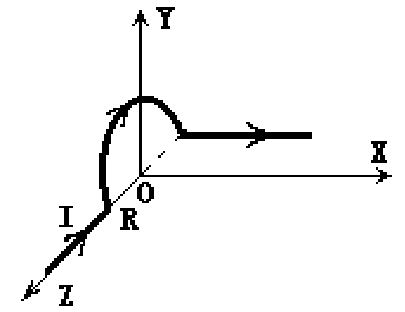
\includegraphics[width=0.18\linewidth]{image/图片16}
	\caption{}
	\label{fig:16}
\end{figure}
	\end{exercise}
	\begin{exercise}
		如图所示,三条无限长直导线平行等距并排放置,导线1、2、3分别通有1A、2A、3A的电流。导线1、2、3单位长度受力分别用$F_{1}$、$F_{2}$、$F_{3}$表示,则          $F_{1}$:$F_{2}$=             ;                $\oint_L{\overrightarrow{B}\cdot d\overrightarrow{l}}$ =? 	          
\begin{figure}[H]
	\centering
	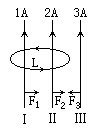
\includegraphics[width=0.18\linewidth]{image/图片17}
	\caption{}
	\label{fig:17}
\end{figure}
	\end{exercise}
	\begin{exercise}
		带电量为$q$的点电荷作半径为$R$的匀速圆周运动,角速度为$\omega$。电荷运动产生的环形电流的电流强度$I =$?,环形电流中心处磁感应强度大小$B =$?,磁矩大小$m $=?
	\end{exercise}
	\begin{exercise}
		半径为$R$的单匝平面圆线圈通有电流$I$,若将该导线弯成匝数$N=2$的平面圆形线圈,导线长度不变,并通以同样的电流。线圈中心的磁感应强度是原来的?倍,线圈的磁矩是原来的?倍
	\end{exercise}
	\begin{exercise}
		无限长直导线弯成图示(a)(b)两种形状,(a)在$P$点处弯成半径为R的圆,(b)在$P$点处弯成边长为$\sqrt{2}R$的正方形。当长直导线通以电流$I$时,分别求两图中O处的磁感应强度。
		
		
\begin{figure}[H]
	\centering
	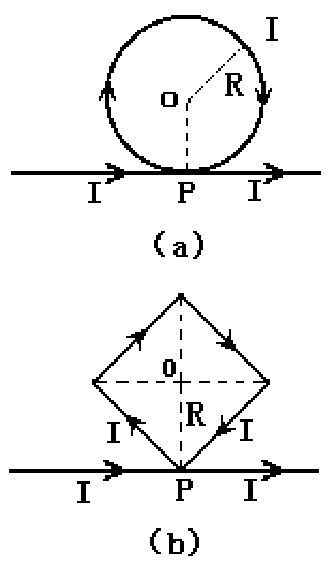
\includegraphics[width=0.18\linewidth]{image/图片18}
	\caption{}
	\label{fig:18}
\end{figure}
	\end{exercise}
	\begin{exercise}
		研究受控热核反应的托卡马克装置中,用螺绕环产生的磁场来约束其中的等离子体。某一托卡马克装置中环管轴线的半径为2.0m,环管截面的半径为1.0m,环管上均匀绕有10km长的水冷铜线。铜线通过峰值为7.3$\times
		$$10^{4}$A的脉冲电流时,环管中心的磁感应强度的峰值是多少?(近似地按恒定电流计算。)
	\end{exercise}
	\begin{exercise}
		如图所示,一无限长导体薄片,宽度为$a$,厚度不计,均匀通有电流$I$,在距它边缘为$a$处平行且共面地放置一条无限长通有同向等值电流的导线。求导线单位长度受到的磁力。
		
		
\begin{figure}[H]
	\centering
	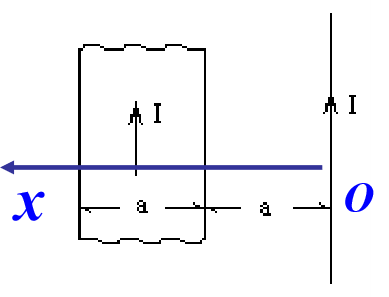
\includegraphics[width=0.18\linewidth]{image/图片19}
	\caption{}
	\label{fig:19}
\end{figure}
	\end{exercise}
	\begin{exercise}
		一长直导线载有电流$I_{1}$,在它的旁边有一等边直角三角形ABC,通有恒定电流$I_{2}$,长直导线与三角形在同一平面内,三角形的直角边AB长为L与导线平行,A点和长直电流相距为$a$,如图示。求:电流$I_{1}$作用于载流导线AB、BC、AC的安培力的大小及方向
		
\begin{figure}[H]
	\centering
	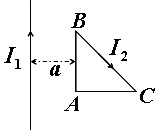
\includegraphics[width=0.18\linewidth]{image/图片20}
	\caption{}
	\label{fig:20}
\end{figure}
		
	\end{exercise}
	\begin{exercise}
		若质子和电子都在垂直于同一磁场的平面内做半径相同的圆周运动,它们的质量分别为$m_{p}$和$m_{e}$,求
		
		(1)质子和电子的动量之比;
		
		(2)质子和电子的动能之比;
		
		(3)质子和电子的绕行周期之比;
	\end{exercise}
	\begin{exercise}
		如图,边长为$a$的等边三角形,通过电流为$I$,放在磁感应强度为$B$的均匀磁场中,磁感方向与线圈平行,当线圈在磁力矩作用下转过180度时,磁力矩所用的功为?
		
\begin{figure}[H]
	\centering
	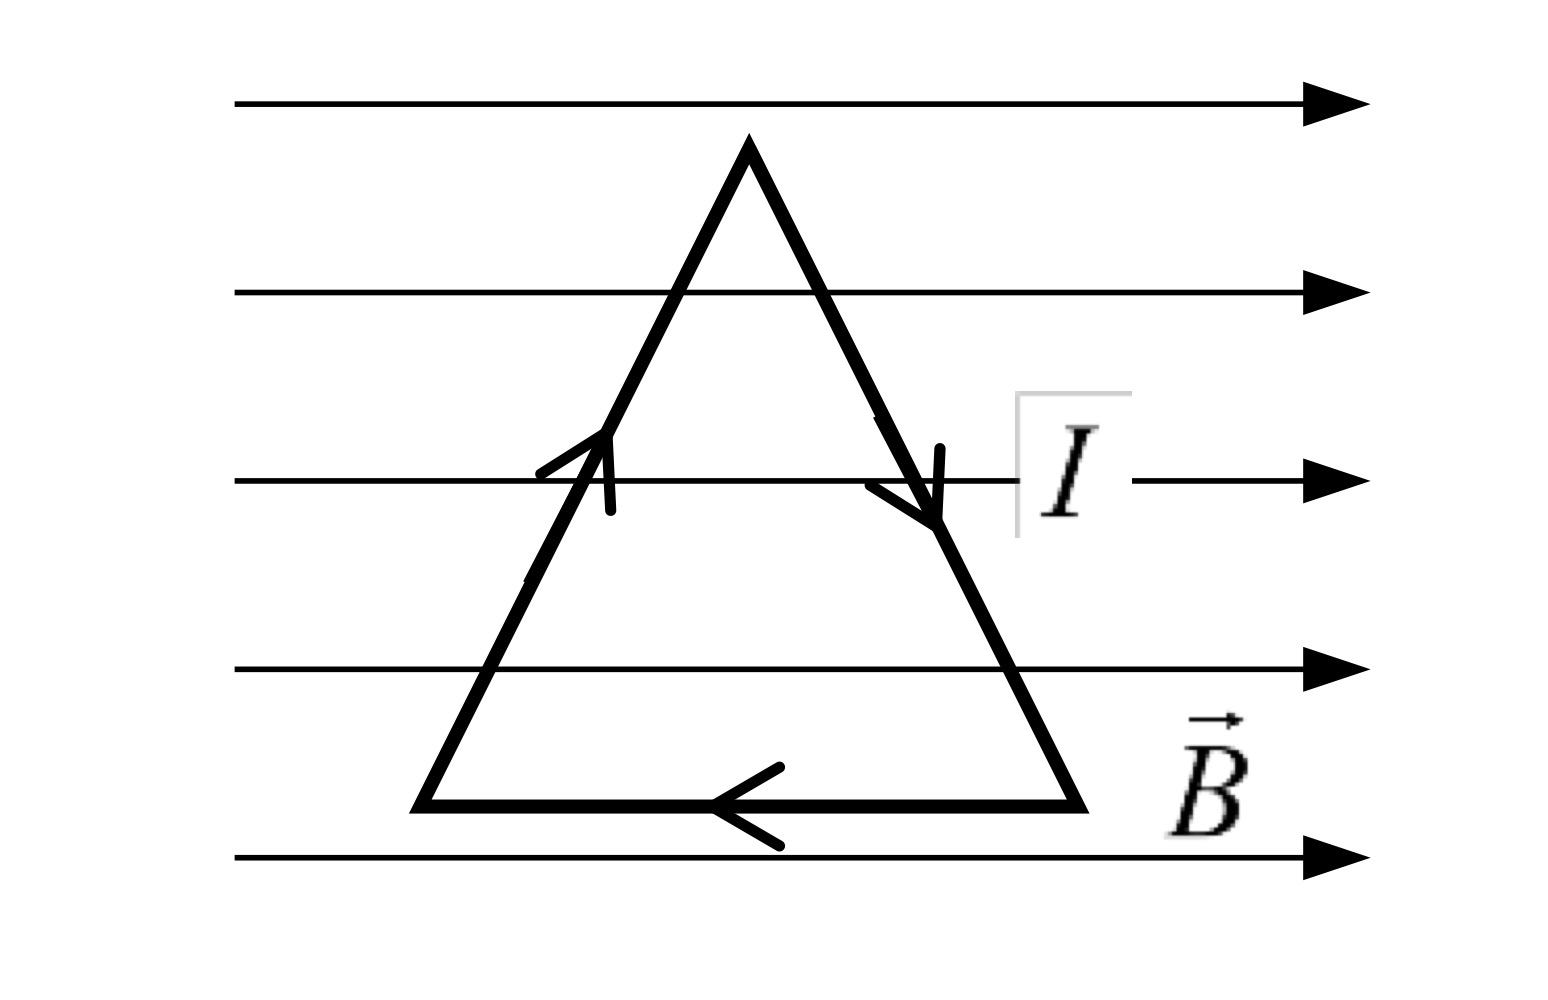
\includegraphics[width=0.18\linewidth]{image/IMG_0435(20231123-215628)}
	\caption{}
	\label{fig:img043520231123-215628}
\end{figure}
	\end{exercise}
	\begin{exercise}
		将一根导线折成正$n$边形,其外接圆半径为$a$,设导线载有电流$I$,如图所示。试求:
		
		(1)外接圆中心处磁感应强度;
		
		(2)当n$\rightarrow \infty$时,上述结果又如何?
		
\begin{figure}[H]
	\centering
	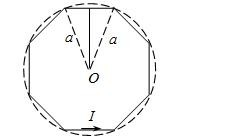
\includegraphics[width=0.18\linewidth]{image/1700748294679}
	\caption{}
	\label{fig:1700748294679}
\end{figure}
		
	\end{exercise}
	\chapter{电磁感应}
	\section{电磁感应}
	
	\begin{introduction}
		\item 感生电动势(重要)
		\item 动生电动势(重要)
	\end{introduction}
	这一部分,又回到了我们亲爱的高中题目,这里只罗列公式,想知道具体内容过一下ppt
	\subsection{\color{red}\text{感生电动势}}
	对于感生电动势,我们有以下公式
	\begin{equation*}
		\varepsilon =-\frac{d\varPhi}{dt}=-\oint_L{\overrightarrow{E}\cdot d\overrightarrow{l}}=-\int{\frac{\partial \overrightarrow{B}}{\partial t}d\overrightarrow{S}}
	\end{equation*}
	\begin{remark}
		其方向用右手定则判断
	\end{remark}
	\begin{remark}
		涡旋电场的内容,稍微过一下ppt就行了
	\end{remark}
	\subsection{\color{red}\text{动生电动势}}
	对于动生电动势,我们有以下公式
	\begin{equation*}
		\varepsilon =\oint_L{\overrightarrow{v}\times \overrightarrow{B}\cdot d\overrightarrow{l}}
	\end{equation*}
	\begin{remark}
		电流方向用右手定则判断
	\end{remark}
	\begin{remark}
		电动势方向从负极到正极
	\end{remark}
	\section{自感与互感}
	\begin{introduction}
		\item 自感与互感(重要)
		\item 自感磁能与互感磁能(重要)
		\item 麦克斯韦方程组(重要)
	\end{introduction}
	 \subsection{\color{red}\text{自感与互感}}
	 \begin{definition}[互感与自感]
	 	一个回路的电流发生变化时,在另一个回路中产生感应电动势,我们称之为互感,用公式表示即为
	 	\begin{equation*}
	 		\varepsilon =-M\frac{dI}{dt},\text{其中}M\text{为互感系数}
	 	\end{equation*}
	 	
	 	同理,自感的公式表达式为
	 	\begin{equation*}
	 		\varepsilon =-L\frac{dI}{dt},\text{其中}M\text{为自感系数}
	 	\end{equation*}
	 \end{definition}
	 \begin{remark}
	 	$M=\frac{\varPhi _2}{I_1}=\frac{\varPhi _1}{I_2}$
	 \end{remark}
	 \begin{remark}
	 	$L=\frac{\varPhi}{I}$
	 \end{remark}
	 \subsection{\color{red}\text{自感磁能与互感磁能}}
	 见《电磁感应》ppt 48页~54页
	 \subsection{\color{red}\text{麦克斯韦方程组}}
	 这一部分的话,我们要知道麦克斯韦方程组的积分形式和微分形式
	 
	 首先是积分形式
	\begin{equation*}
		\begin{split}
			1.\text{电场高斯定理:}\ointclockwise{\overrightarrow{D}\cdot d\overrightarrow{S}}=\iiint{\rho _0dV}=Q\left( \text{电场是有源场,电荷总是伴随着电场} \right) 
			\\
			2.\text{磁场高斯定理:}\ointclockwise{\overrightarrow{B}\cdot d\overrightarrow{S}}=0\left( \text{磁场是无源场,磁力线闭合} \right) 
			\\
			3.\text{全电流安培环路定理:}\ointclockwise{\overrightarrow{H}\cdot d\overrightarrow{l}}=I+I_d=\iint{\overrightarrow{j_{0}}d\overrightarrow{S}}+\iint{\frac{\partial \overrightarrow{D}}{\partial t}d\overrightarrow{S}\left( \text{变化的电场产生磁场} \right)}
			\\
			4.\text{安培环路定理:}\ointclockwise{\overrightarrow{E}\cdot d\overrightarrow{l}}=-\frac{d\varPhi}{dt}=-\iint{\frac{\partial \overrightarrow{B}}{\partial t}}d\overrightarrow{S}\left( \text{变化的磁场一定伴随着电场} \right)  
		\end{split}
	\end{equation*}
	 \begin{remark}
	 	$I_{d}$为位移电流,当电容器充、
	 	放电时,电容器中的电场发生变化,变化的电场可等
	 	效为电流,这种电流称为位移电流
	 \end{remark}
	 
	 同样,我们可得到麦克斯韦方程组的微分形式
	 \begin{equation*}
	 	\begin{split}
	 		1.\text{电场高斯定理:}\overrightarrow{\nabla }\cdot \overrightarrow{D}=\rho _0
	 		\\
	 		2.\text{磁场高斯定理:}\overrightarrow{\nabla }\cdot \overrightarrow{B}=0\left( \text{磁场是无源场,磁力线闭合} \right) 
	 		\\
	 		3.\text{全电流安培环路定理:}\overrightarrow{\nabla }\times \overrightarrow{H}=\overrightarrow{j_0}+\frac{\partial \overrightarrow{D}}{\partial t}
	 		\\
	 		4.\text{安培环路定理:}\overrightarrow{\nabla }\times \overrightarrow{E}=-\frac{\partial \overrightarrow{B}}{\partial t}
	 	\end{split}
	 \end{equation*}
	 这些东西,请务必要记住
	 \section{习题训练}
	 \begin{exercise}
	 	如图所示,直角三角形金属框架ABC放在均匀磁场中,磁场$B_{0}$平行于AB边,AC的长度为l,当金属框架绕AB边以匀角速度$\omega$转动时,ABC回路中的感应电动势$\varepsilon$和B、C两点间的电势差$U_{B}-U_{C}$为 ?
	 	
\begin{figure}[H]
	\centering
	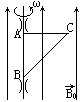
\includegraphics[width=0.18\linewidth]{image/图片21}
	\caption{}
	\label{fig:21}
\end{figure}
	 	
	 \end{exercise}
	 \begin{exercise}
	 	圆柱形区域内存在一匀强磁场$B$,且以恒定变化率$\frac{dB}{dt}$减小,一边长为l的正方形导体框abcd置于该磁场中,框平面与磁场垂直,如图所示,a、c处的感生电场强度大小$E_{ka}=$?、$E_{kc}=$?;bc段上的感生电动势大小$\varepsilon_{bc}$=?;cd段上的感生电动势大小$\varepsilon_{cd}$=?;回路的总感生电动势大小$\varepsilon_{i}$=?
	 	
\begin{figure}[H]
	\centering
	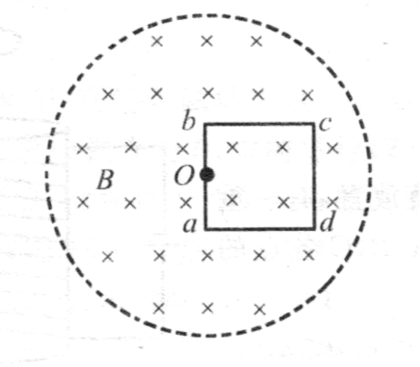
\includegraphics[width=0.18\linewidth]{image/图片22}
	\caption{}
	\label{fig:22}
\end{figure}
	 	
	 \end{exercise}
	 \begin{exercise}
	 	载有恒定电流I的长直导线旁有一半圆环导线cd, 半圆环半径为$R$,环面与直导线垂直,且半圆环两端点连线的延长线与直导线相交,如图所示。当半圆环以速率$v$沿平行于直导线的方向平移时,半圆环上的感应电动势的大小?
	 	
\begin{figure}[H]
	\centering
	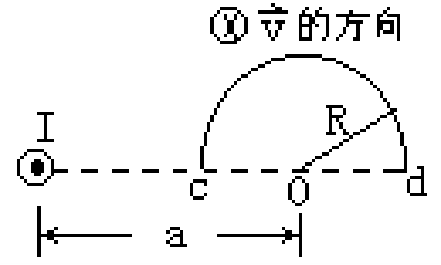
\includegraphics[width=0.18\linewidth]{image/图片23}
	\caption{}
	\label{fig:23}
\end{figure}
	 \end{exercise}
	 \begin{exercise}
	 	无限长直导线旁有一与其共面的矩形线圈,直导线中通有恒定电流$I$,将此直导线及线圈共同置于随时间变化的而空间分布均匀的磁场$B$中,设$\frac{dB}{dt}$>0,当线圈以速度$v$垂直长直导线向右运动时,求线圈在如图所示位置时的感应电动势
	 	
\begin{figure}[H]
	\centering
	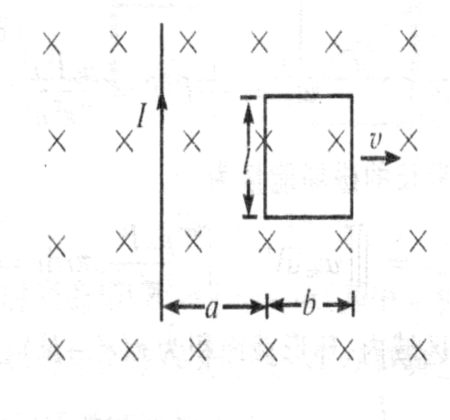
\includegraphics[width=0.18\linewidth]{image/图片24}
	\caption{}
	\label{fig:24}
\end{figure}
	 	
	 \end{exercise}
	 \begin{exercise}
	 	一个单位长度上绕有$n_{1}$匝线圈的空心长直螺线管的自感系数为$L_{1}$,另一个单位长度上绕有$n_{2}=2n_{1}$匝线圈的空心长直螺线管的自感系数为$L_{2}$,已知二者的横截面积和长度均相同,则$L_{1}$与$L_{2}$的关系为
	 \end{exercise}
	 \begin{exercise}
	 	两根相距$d$的平行长直导线与电源组成回路,已知回路电流为$I$,导线截面半径为$r_{0}$,$L$表示两导线回路的单位长度的自感,则沿导线单位长空间内的自感磁场能量为 
	 \end{exercise}
	 \begin{exercise}
	 	一环形螺线管,在磁导率为$\nu$ 的磁介质上绕有$N$匝线圈。磁介质截面为长方形,尺寸如图所示。用能量法求螺线管的自感系数
	 	
\begin{figure}[H]
	\centering
	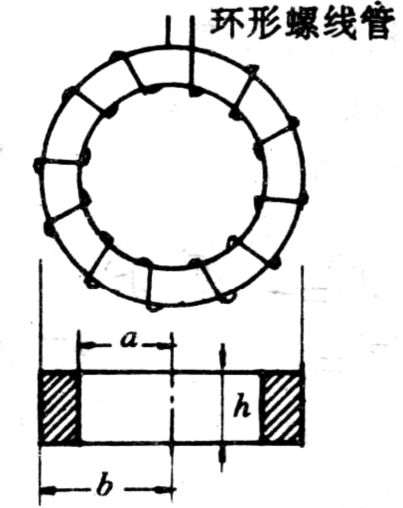
\includegraphics[width=0.18\linewidth]{image/图片25}
	\caption{}
	\label{fig:25}
\end{figure}
	 	
	 \end{exercise}
	 \begin{exercise}
	 	边长分别为a和b的两个正方形线圈如图所示放置在同一平面内,大线圈的电流在小线圈处产生的磁场近似均匀。
	 	
	 	(1)求两线圈间的互感系数;
	 	
	 	(2)若大线圈中的电流按$I=I_{0}\sin(\omega t)$的规律变化,求小线圈中的互感电动势
	 	
\begin{figure}[H]
	\centering
	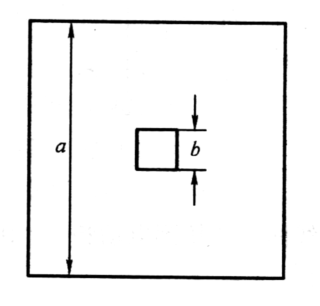
\includegraphics[width=0.18\linewidth]{image/图片26}
	\caption{}
	\label{fig:26}
\end{figure}
	 	
	 \end{exercise}
	 \begin{exercise}
	 	长为$l$的导体棒,如图所示放在均匀磁场中,棒与磁场垂直,当棒以速度$v$平行于参考线向右运动时,棒两端的动生电动势$\varepsilon_{ab}$为?;导体棒中非静电性电场的强度为?、方向为?
	 	
\begin{figure}[H]
	\centering
	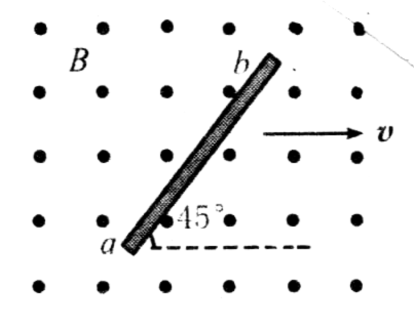
\includegraphics[width=0.18\linewidth]{image/图片27}
	\caption{}
	\label{fig:27}
\end{figure}
	 	
	 \end{exercise}
	 \begin{exercise}
	 	如图所示,在半径为$R$的圆柱空间内有均匀磁场$B$,一金属棒如图放置。若磁场随时间增强,$\frac{dB}{dt}=a$($a$为大于零的常量),则棒两端的感应电动势大小为?,?端电势高
	 	
\begin{figure}[H]
	\centering
	\includegraphics[width=0.18\linewidth]{image/图片28}
	\caption{}
	\label{fig:28}
\end{figure}
	 	
	 \end{exercise}
	 \begin{exercise}
	 	在某个电子感应加速器中,从上向下看时,电子沿逆时针方向旋转,如图所示,则电子正在加速运动时,加速器中磁场的方向?;磁场的磁感应强度随时间?(填增加或减小)
	 	
\begin{figure}[H]
	\centering
	\includegraphics[width=0.18\linewidth]{image/图片29}
	\caption{}
	\label{fig:29}
\end{figure}
	 	
	 \end{exercise}
	 \begin{exercise}
	 	圆形平行板电容器,极板半径为$R$。在放电过程中某一时刻的电流为$I_{0}$,则此时电容器中位移电流密度大小$j_{d}$ =?;距电容器中心为$r$的$P$点处的磁场强度大小$H =$?
	 \end{exercise}
	 \begin{exercise}
	 	无限长直导线同平面放置正方形导线圈ABCD,如图所示。正方形边长为$a$,AB和长直导线相距为$b$,则二回路的互感系数为                 
\begin{figure}[H]
	\centering
	\includegraphics[width=0.18\linewidth]{image/图片30}
	\caption{}
	\label{fig:30}
\end{figure}
	 \end{exercise}
	 \begin{exercise}
	 	如图所示,长为L的金属棒置于无限长直电流I产生的磁场中,金属棒与长直电流共面,并在此平面内绕其一端O以匀角速度$\omega$做顺时针旋转,O端与长直电流的距离为d。求金属棒转至下述两种位置时产生的感应电动势:
	 	
	 	(1)转至OA位置;
	 	
	 	(2)转至OB位置。
	 	
\begin{figure}[H]
	\centering
	\includegraphics[width=0.18\linewidth]{image/图片31}
	\caption{}
	\label{fig:31}
\end{figure}
	 	
	 \end{exercise}
	 \begin{exercise}
	 	一同轴电缆由半径为$R_{1}$的中心导体圆柱和半径为$R_{2}$的外层导体圆筒组成,二者之间充满磁介质,磁介质和金属的相对磁导率均可看作1。当电缆通过电流$I$(由中心圆柱流出,由外层圆筒流回)时,单位长度电缆储存的磁场能量是多少?利用自感磁能公式求出单位长度电缆的自感系数
	 	
\begin{figure}[H]
	\centering
	\includegraphics[width=0.18\linewidth]{image/图片32}
	\caption{}
	\label{fig:32}
\end{figure}
	 	
	 \end{exercise}
	 \begin{exercise}
	 	两长直螺线管的长度分别为$l_{a}$和$l_{b}$,自感分别为$L_{a}$和$L_{b}$,截面近似相等,均匀密绕,绕向相同。
	 	
	 	(1)计算两螺线管的互感;
	 	
	 	(2)若回路$a$闭合,电阻近似为零,回路$b$中通有电流$I_{b}=kt$,计算$a$中的电流
	 	
	 	
\begin{figure}[H]
	\centering
	\includegraphics[width=0.18\linewidth]{image/图片33}
	\caption{}
	\label{fig:33}
\end{figure}
	 \end{exercise}
	 \begin{exercise}
	 	图中所示为靠近放置的两线圈,自感分别为$L_{1}$=4.0mH,$L_{2}$=8.0mH,若把线端2与线端3相连接,测得1、4间的总自感L=6.0mH。问:若把线端2与端4相连接,则1、3间的总自感将为多少
	 	
\begin{figure}[H]
	\centering
	\includegraphics[width=0.18\linewidth]{image/图片34}
	\caption{}
	\label{fig:34}
\end{figure}
	 	
	 \end{exercise}
	\chapter{证明题专栏}
	\begin{exercise}
		试证明静电场电场线永不闭合
	\end{exercise}
	\begin{exercise}
		若穿过闭合曲面$S$的磁通量为零,能不能肯定面上各点的场强都为零?
	\end{exercise}
	\begin{exercise}
		电势为零处,场强一定为零,这种说法正确吗?请举例说明你的看法
	\end{exercise}
	\begin{exercise}
		写出Maxwell电磁理论的两个重要假说和Maxwell方程组的积分形式,并
		说明它们与静止场和稳定场中的形式有何本质区别。两个重要预言是什么。
	\end{exercise}
	\begin{exercise}
		场强大小相等的地方,电势是否相等?等势面上的场强是否相等?
	\end{exercise}
	\begin{exercise}
		一个带电的导体A在接近接地的导体B时,导体B是否保持原电势?
	\end{exercise}
	\begin{exercise}
		电场线是否能在无电荷处中断?为什么?
	\end{exercise}
	\begin{exercise}
		变化的磁场所激发的电场是否一定随时间而变化,为什么?
	\end{exercise}
\end{document}